%-------------------------------------------------------------------------------
\section{Einführung in die Vorlesung}
%-------------------------------------------------------------------------------

%%% Folie
{
\scriptsize

\begin{frame}{Inhalte der Vorlesung}
    \begin{columns}
        \begin{column}[T]{.7\textwidth}
            \begin{block}{Übergeordnete Lernziele}
                \begin{itemize}
                    \item Die vorhandenen Programmierkenntnisse praktisch anwenden können
                    \item Eingebettete IoT-Anwendungen in Python programmieren können
                    \item Für IoT-Anwendungen nützliche Python-Bibliotheken nutzen können
                    \item Nach Bibliotheken suchen und sich in diese einarbeiten können
                \end{itemize}
            \end{block}

            \begin{block}{Themenschwerpunkte}
                \begin{itemize}
                    %~ \item Definition und Architektur des Internet of Things
                    %~ \item Ansteuerung von Hardwarebausteinen über den GPIO-Port
                    %~ \item Datenaustausch in verteilten IoT-Systemen
                    %~ \item Ablage von Messwerten und Sensordaten in einer Datenbank
                    %~ \item Visualisierung und Auswertung der gespeicherten Sensordaten
                    \item Grundlagen des Internet of Things
                    \item Hardwarenahe Programmierung in Python
                    \item Datenauschtausch in verteilten IoT-Systemen
                    \item Messwerte und Sensordaten speichern
                    \item Daten visualisieren und auswerten
                \end{itemize}
            \end{block}
        \end{column}

        \begin{column}[T]{.3\textwidth}
            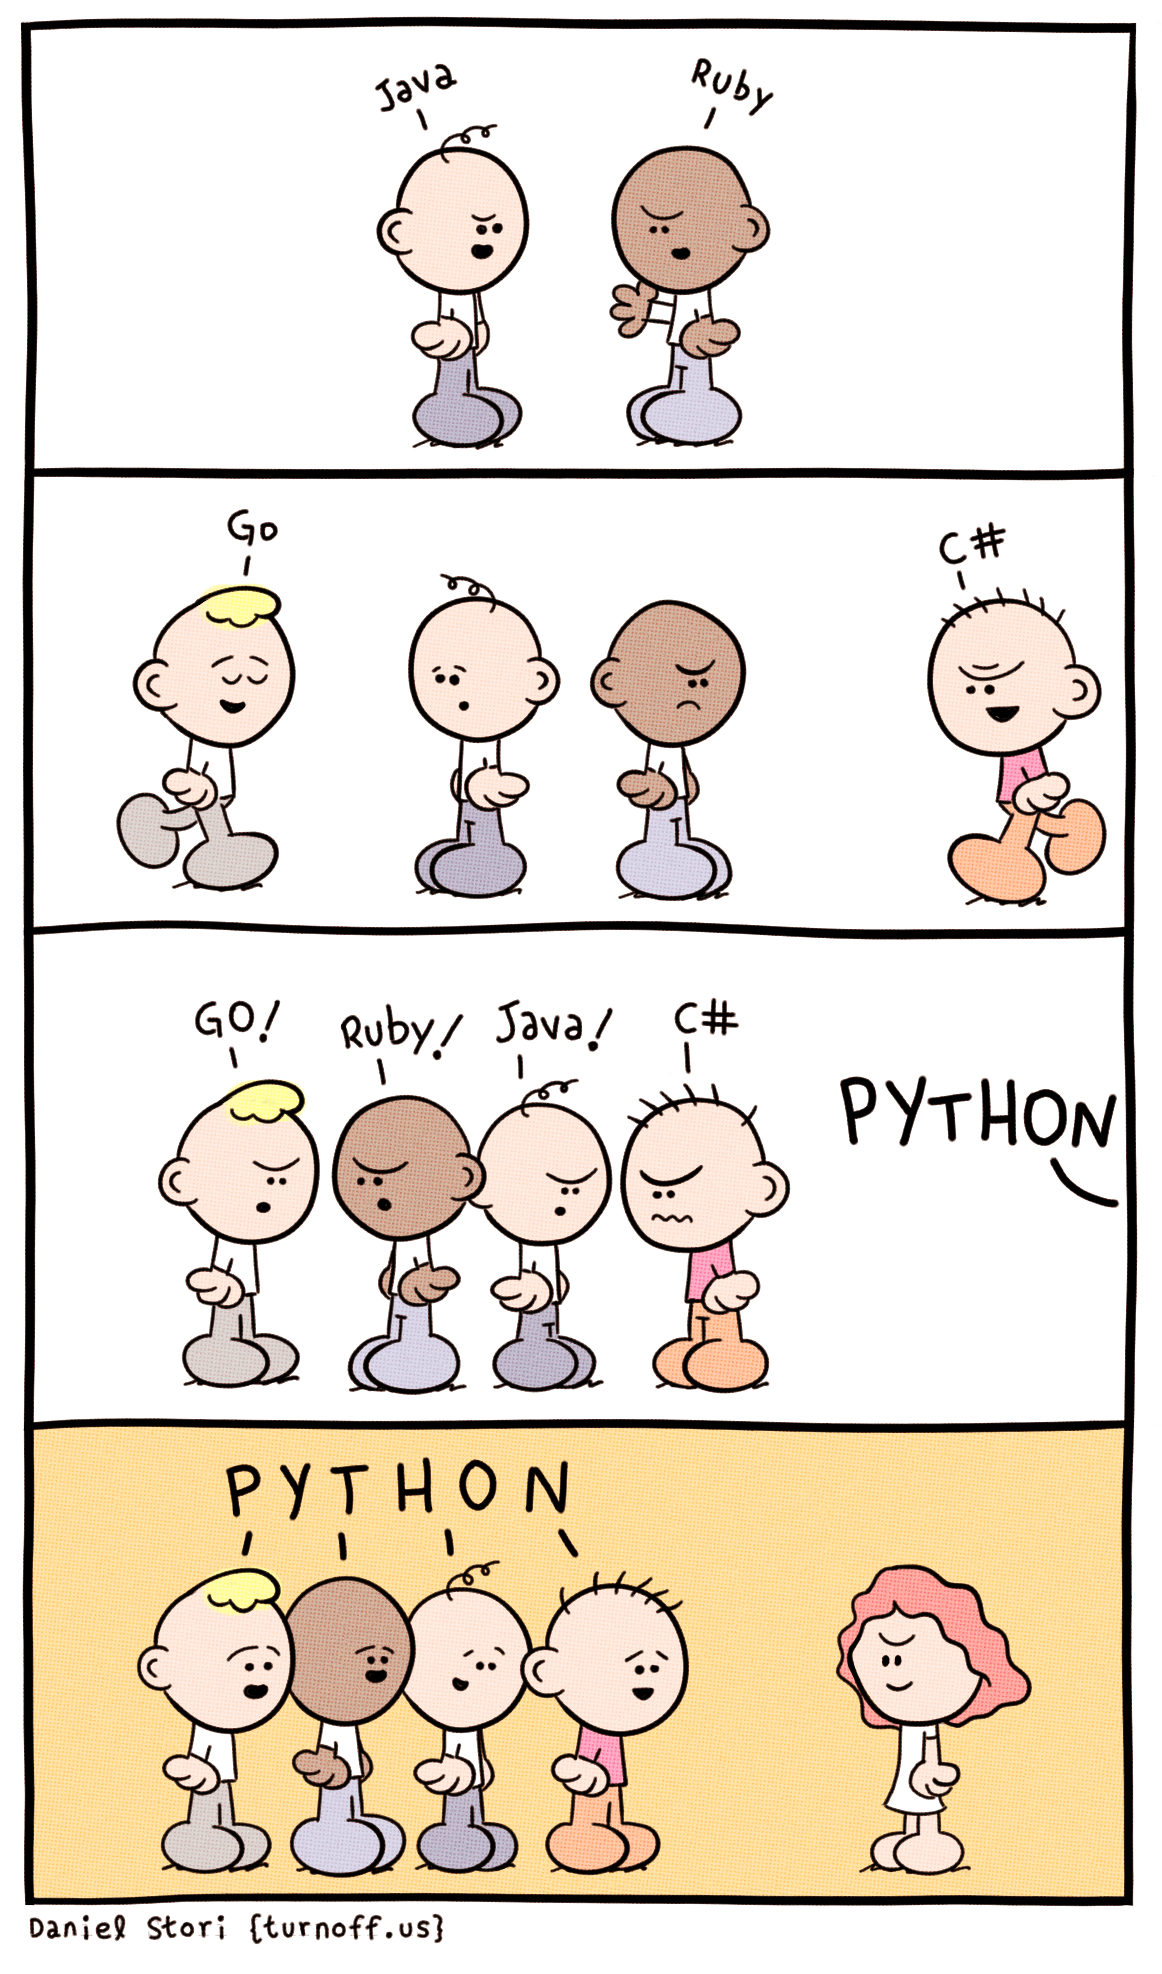
\includegraphics[width=\textwidth]{img/depressed-developer-35}
        \end{column}
    \end{columns}
\end{frame}
}

{
\footnotesize

%%% Folie
\begin{frame}{Didaktisches Modell}
    \begin{columns}
        \begin{column}[T]{.5\textwidth}
            \textbf{Ablauf der Vorlesungsstunden}
            \medskip

            \begin{enumerate}
                \item Fragen und Wiederholung
                \item Besprechung des jeweiligen Themas
                \item Entwicklung eines Fallbeispiels
                \item Bekanntgabe der Übungsaufgaben
            \end{enumerate}
        \end{column}

        \begin{column}[T]{.5\textwidth}
            \textbf{Prüfungsleistung}
            \medskip

            \begin{enumerate}
                \item 50\% Übungsaufgaben
                \item 50\% Praktische Aufgabe
            \end{enumerate}
        \end{column}
    \end{columns}

    \vfill
    \Justified{
        \scriptsize
        Zusätzlich werden wir ein paar Übungsstunden einbauen, wobei die Aufgaben
        auch außerhalb der Stunden eigenständig bearbeitet werden sollen. Rückfragen
        können deshalb über die Vorlesung hinaus auch per Mail an
        \textcolor{RoyalPurple}{%
            \href{mailto:"Dennis Schulmeister-Zimolong" <dhbw@windows3.de>}{dhbw@windows3.de}%
        }
        geklärt werden.

        \smallskip
        Ein Teil der Lösungen wird am Semesterende zur Benotung abgegeben. Hinzu kommt eine
        praktische Programmieraufgabe in der zweiten Hälfte des Semesters.
    }
\end{frame}
}

%%% Folie
{
\footnotesize

\begin{frame}{Benötigte Hard- und Software}
        \begin{columns}
            \begin{column}[T]{.5\textwidth}
                \textbf{Hardware}
                \medskip

                \Justified{
                    \scriptsize
                    Für die Vorlesung wurden neue Raspberry Pi bestellt, die kostenlos
                    ausgeliehen werden können. Allerdings wurden sie aufgrund der
                    weltweiten Lieferkettenprobleme noch nicht geliefert. Notfalls
                    werden wir die Hardware einfach mit Python simulieren. \smiley{}
                }
                \medskip

                \begin{itemize}
                    \item Raspberry Pi
                    \item Diverse Sensoren und Aktoren
                \end{itemize}
            \end{column}
            \begin{column}[T]{.5\textwidth}
                \textbf{Software}
                \medskip

                \Justified{
                    \scriptsize
                    Lediglich ein paar Entwicklungswerkzeuge für die Programmierung mit
                    Python sowie die Remote-Entwicklung werden benötigt. Einige Beispiele
                    können auch lokal ohne Raspberry Pi ausgeführt werden, wofür auf Ihrem
                    Laptop ebenfalls Python benötigt wird.
                }
                \medskip

                \begin{itemize}
                    \item Visual Studio Code
                    \item OpenSSH
                    \item Python
                \end{itemize}
            \end{column}
        \end{columns}
\end{frame}
}

%%% Folie
{
\footnotesize
\setlength{\fboxsep}{0pt}

\begin{frame}{Literaturempfehlungen}
    \fbox{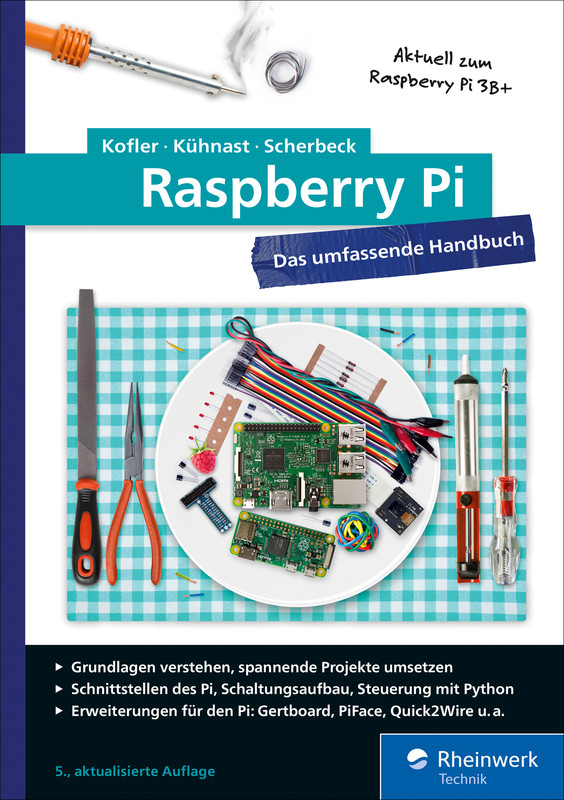
\includegraphics[height=3.3cm]{img/buch_raspberrypi}}
    \hfill
    \fbox{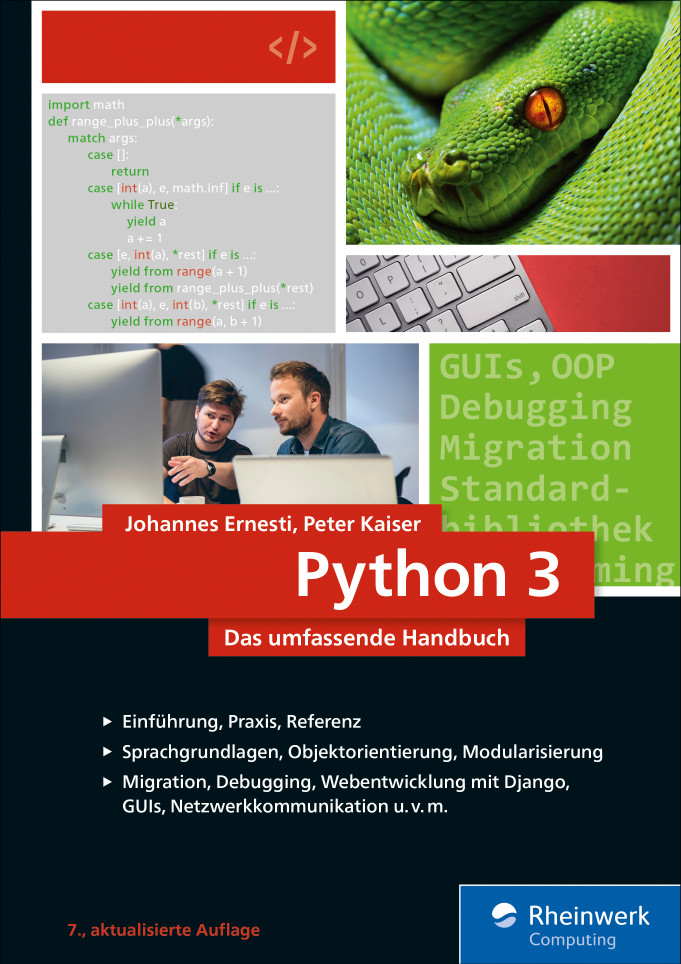
\includegraphics[height=3.3cm]{img/buch_python3_handbuch}}
    \hfill
    \fbox{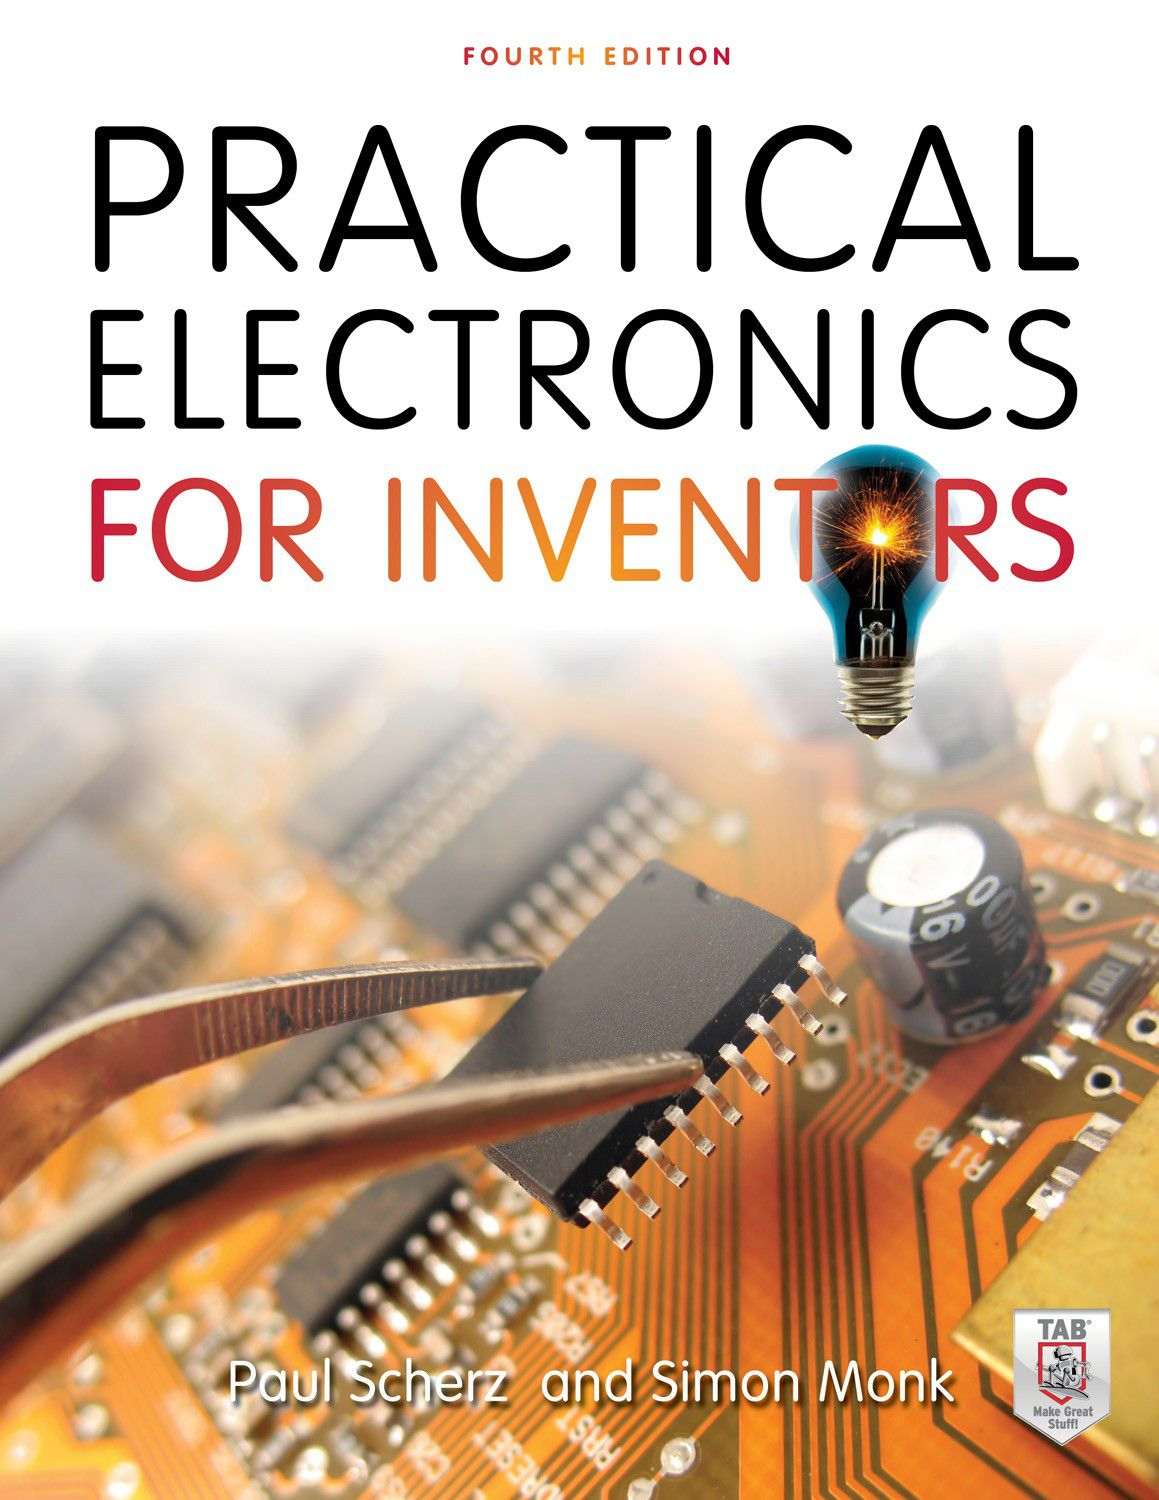
\includegraphics[height=3.3cm]{img/buch_practical_electronics}}
    \hfill
    \fbox{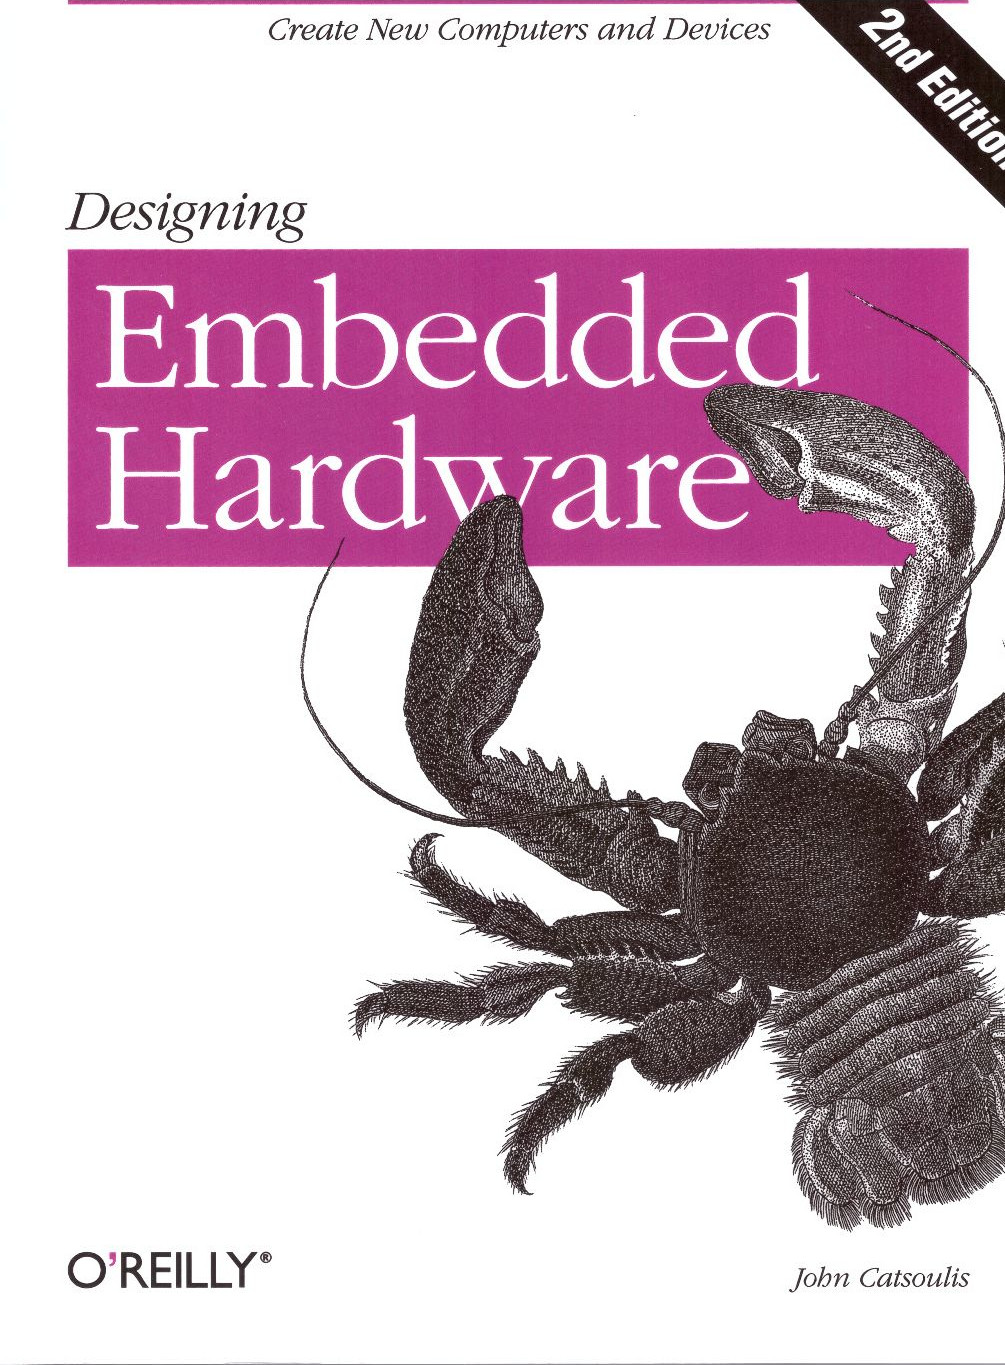
\includegraphics[height=3.3cm]{img/buch_embedded_hardware}}

    \vskip 0.6cm

    \begin{columns}
        \column[T]{.5\textwidth}
        \textbf{Raspberry Pi: Das umfassende Handbuch} \\ Rheinwerk Verlag, 2018

        \column[T]{.5\textwidth}
        \textbf{Python 3: Das umfassende Handbuch} \\ Rheinwerk Verlag, 2023
    \end{columns}

    \vskip 0.6cm

    \begin{columns}
        \column[T]{.5\textwidth}
        \textbf{Practical Electronics for Inventors} \\ McGraw-Hill, 2016

        \column[T]{0.5\textwidth}
        \textbf{Designing Embedded Hardware} \\ O'Reilly, 2005
    \end{columns}
\end{frame}
}

%%% Folie
\begin{frame}{Lernziele für heute}
    \begin{itemize}
        \item ,,Internet of Things'' und ,,eingebettete Systeme'' voneinander abgrenzen
        \item Die Bedeutung des Internet der Dinge in der heutigen Zeit verstehen
        \item Aktuelle IoT-Anwendungsfälle und Geschäftsprozesse erkennen
        \item Typische Schichten und Komponenten einer IoT-Architektur benennen
        %\item Den aktuellen Stand der Technik im historischen Kontext einordnen
        \item Die Vielfalt angebotener Single Board Computer einschätzen können
        \item Die Begriffe ,,Microcontroller'' und ,,System-on-a-Chip'' erklären
        %\item Die Anforderungen an eingebettete Hard- und Software verstehen
        \item Die Grundprinzipien der hardwarenahen Programmierung kennen
    \end{itemize}
\end{frame}

%-------------------------------------------------------------------------------
\section{IoT-Anwendungsfälle}
%-------------------------------------------------------------------------------

%%% Folie
\begin{frame}{Ein paar Fragen zum Einstieg}
    \begin{columns}
        \begin{column}[b]{.5\textwidth}
            \begin{center}
                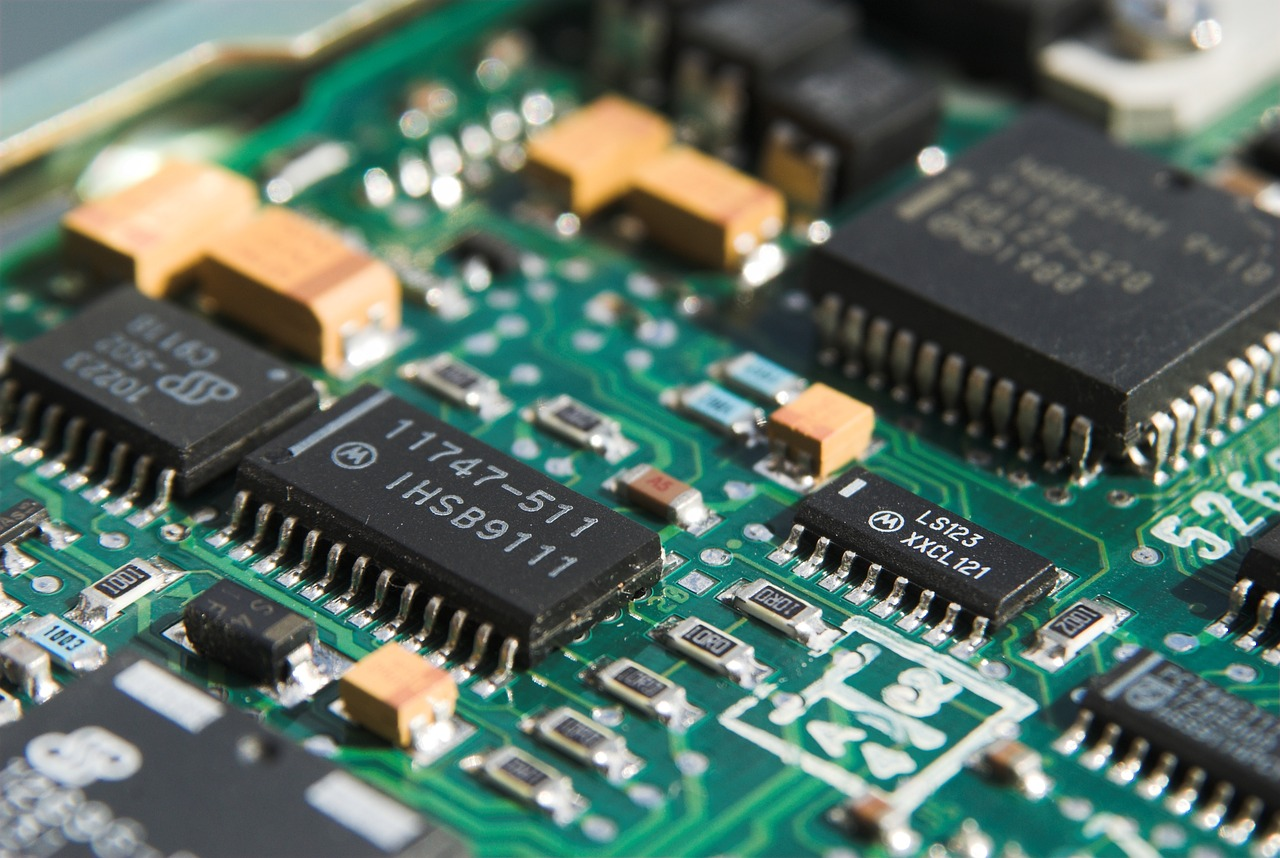
\includegraphics[width=\textwidth]{img/iot-hardware}
            \end{center}
        \end{column}
        \begin{column}[b]{.5\textwidth}
            \begin{center}
                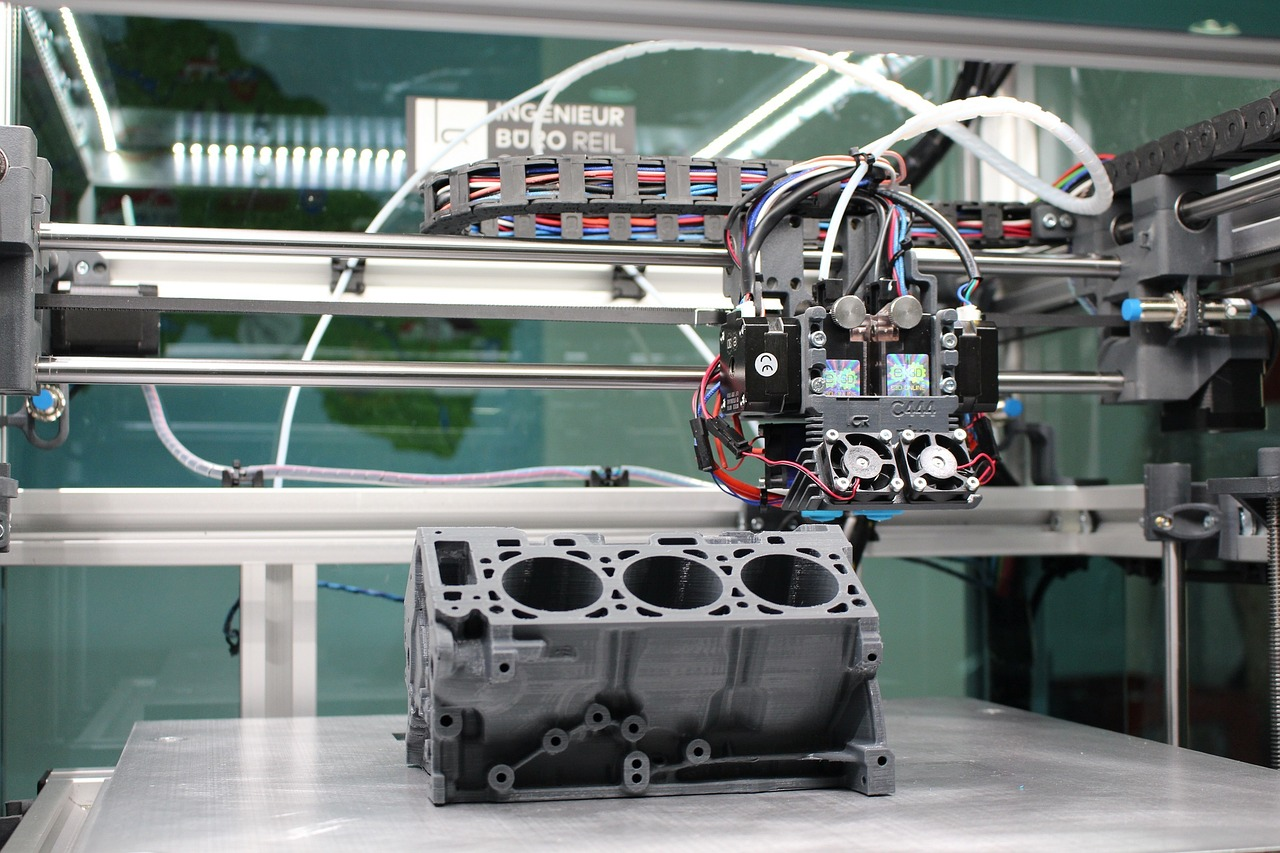
\includegraphics[width=\textwidth]{img/iot-mechatronik}
            \end{center}
        \end{column}
    \end{columns}

    \bigskip

    \begin{itemize}
        \item Was bedeutet der Begriff ,,Eingebettetes System''?
        \item Was bedeutet der Begriff ,,Internet of Things''?
        \item Welche Bedeutung haben sie für die Mechatronik?
        \item Welche Anwendungsfälle können Sie sich vorstellen?
    \end{itemize}
\end{frame}

%%% Folie
{
\footnotesize

\begin{frame}{Definition ,,Eingebettetes Computersystem''}
    \begin{block}{Definition}
        \Justified{
            \smallskip

            Eingebettete Systeme sind kleine Mikrocomputer, die innerhalb eines größeren Geräts
            meist unsichtbar verbaut sind, um seine Funktionen zu steuern und zu überwachen.
            \smallskip

            Ihre grundsätzliche Architektur ist dieselbe wie bei konventionellen Computern,
            jedoch verfügen sie über weitaus weniger, genau auf den Anwendungsfall zugeschnittene
            Ressourcen bei minimalen Kosten, Platzbedarf und Energieverbrauch. Der Leitgedanke
            hierbei lautet ,,so viel wie gerade nötig, so wenig wie absolut möglich''.
            \smallskip

            Eingebettete Systeme sind meist in sich geschlossene Systeme mit deterministischem
            Systemverhalten, die rund um die Uhr laufen und exakt eine Aufgabe erfüllen.
        }
    \end{block}

    \begin{block}{Beispiele}
        \begin{columns}[onlytextwidth]
            \column[b]{.2\textwidth}
            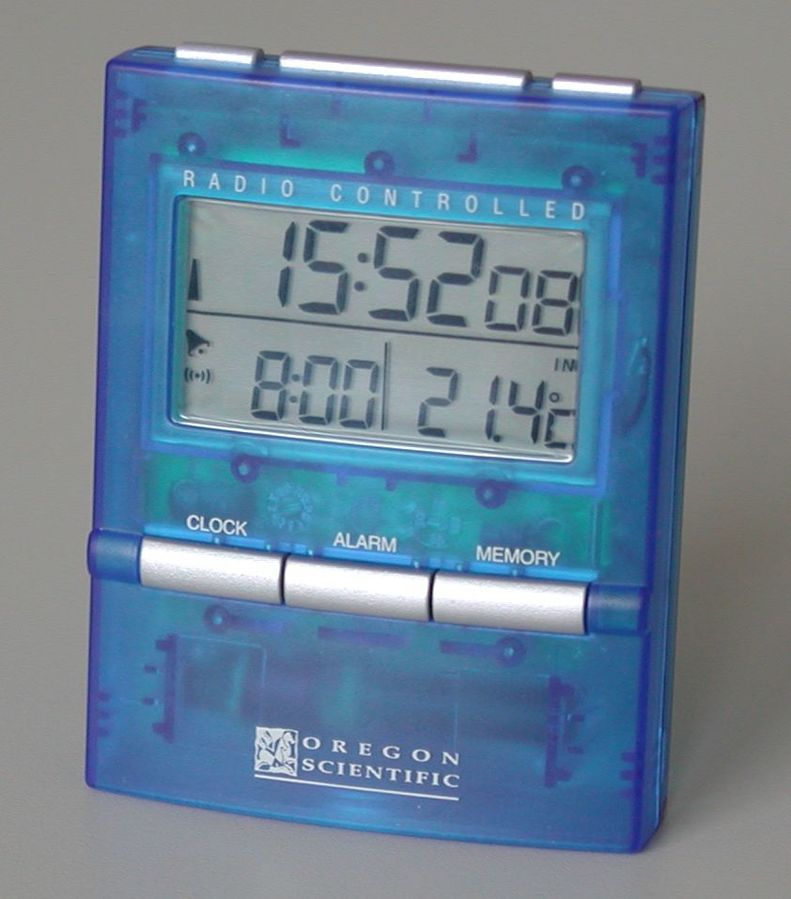
\includegraphics[width=\textwidth]{img/funkwecker}

            \column[b]{.2\textwidth}
            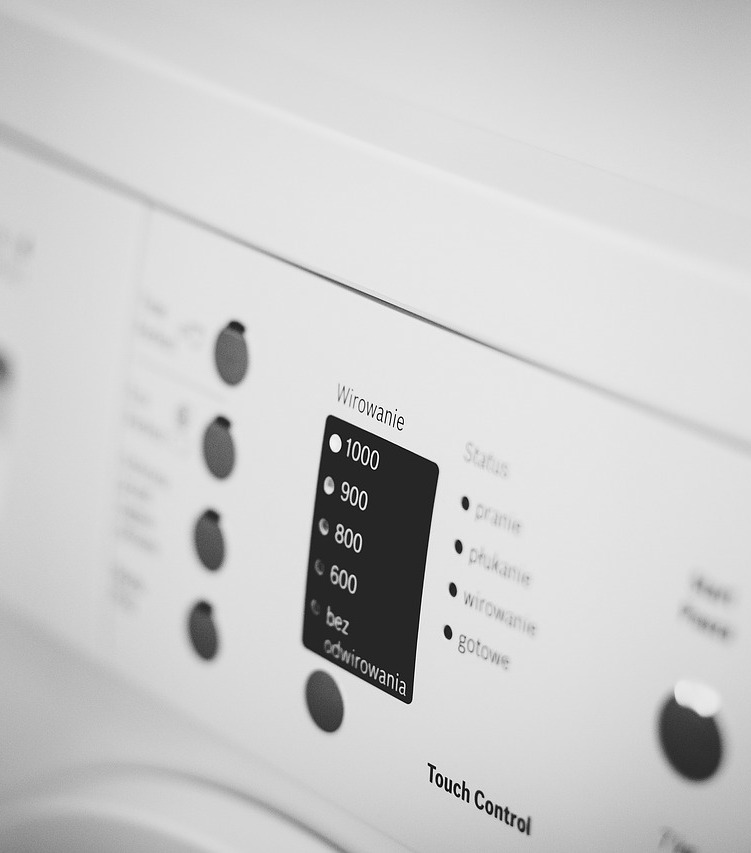
\includegraphics[width=\textwidth]{img/washing-machine-2617514_1280}

            \column[b]{.2\textwidth}
            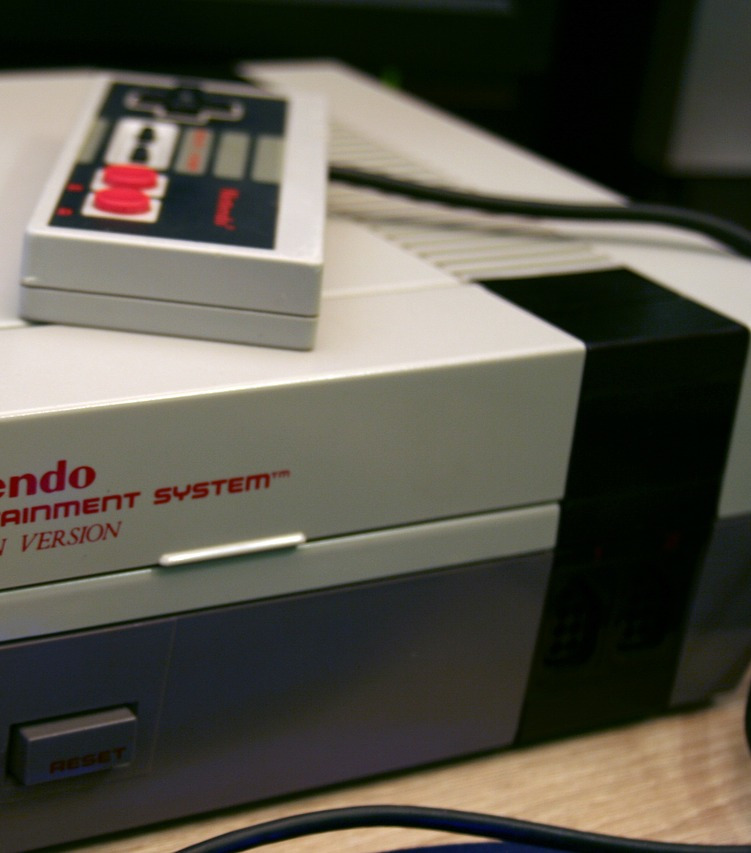
\includegraphics[width=\textwidth]{img/nes-2649705_1280}

            \column[b]{.2\textwidth}
            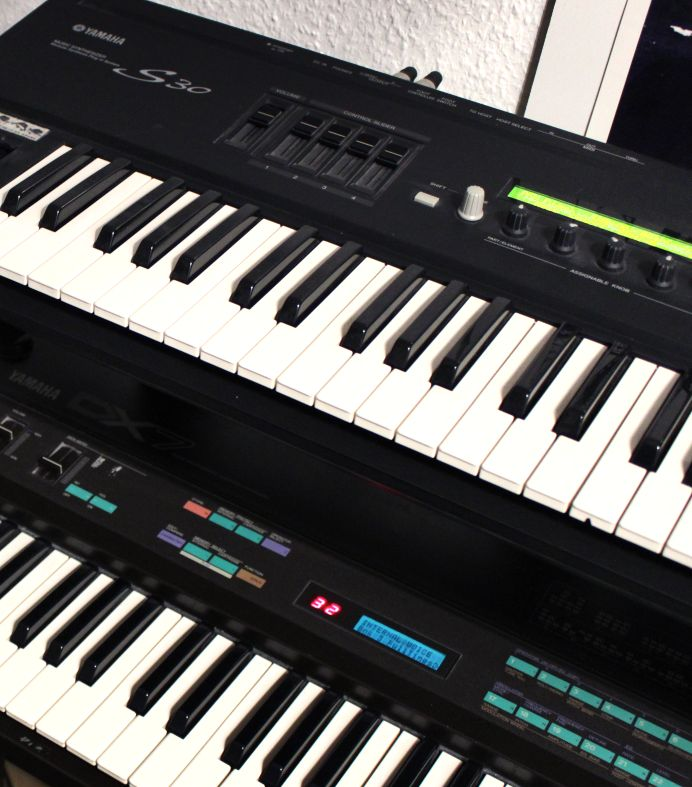
\includegraphics[width=\textwidth]{img/keyboards}

            \column[b]{.2\textwidth}
            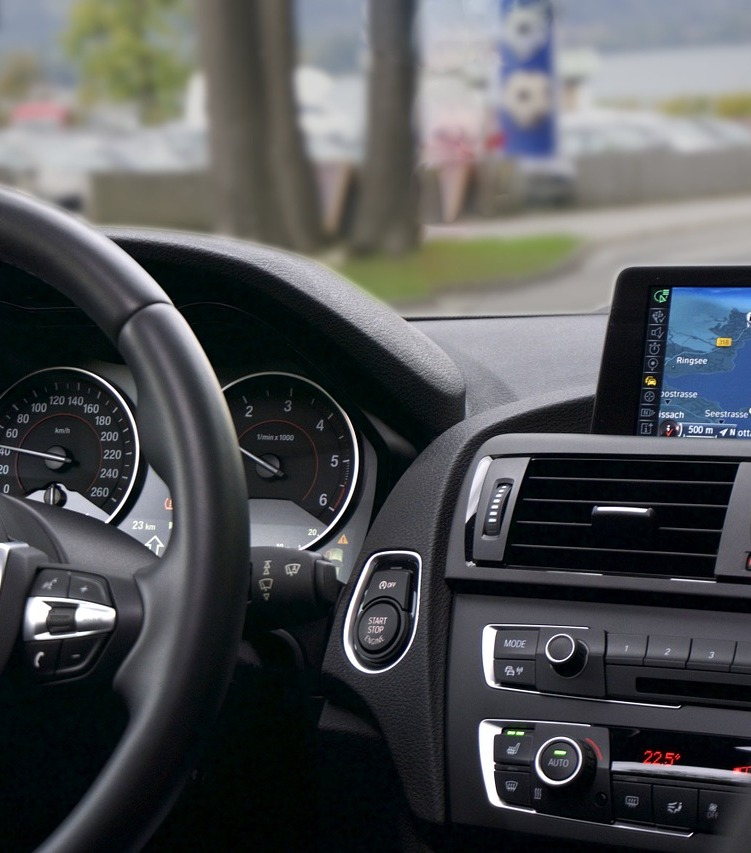
\includegraphics[width=\textwidth]{img/car-1281640_1280}
        \end{columns}
    \end{block}
\end{frame}
}

%%% Folie
{
\footnotesize

\begin{frame}{Definition ,,Internet of Things''}
    \begin{block}{Definition}
        \Justified{
            \smallskip

            IoT-Devices sind eingebettete Systeme größerer Leistungsklasse mit quasi-permanenter
            Internetverbindung.
            \smallskip

            Die ursprüngliche Definition aus dem Jahr 1999 sah die maschinenlesbare Identifikation
            physischer Objekte anhand von RFID-Tags vor. Heute versteht man darunter elektronische
            Geräte mit eingebetteten, mit dem Internet verbundenen Computermodulen, die über eine
            IP-Adresse weltweit eindeutig adressiert werden können.
            \smallskip

            Im erweiterten Sinne zählen zum ,,Internet of Things'' auch Infrastruktur, Cloudplattformen
            und Backendservices, über welche die Devices miteinander verbunden, verwaltet, gesteuert
            und überwacht werden können.
        }
    \end{block}

    \medskip
    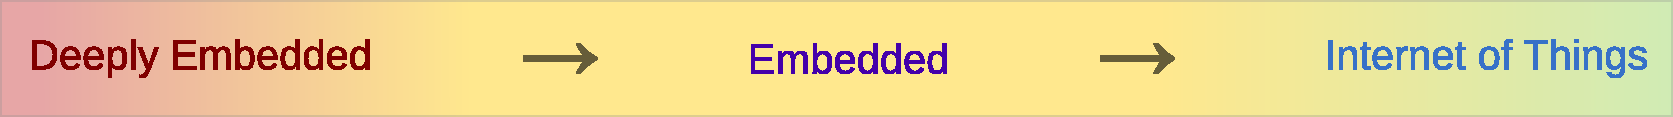
\includegraphics[width=\textwidth]{img/embedded_typen}

    \begin{block}{Beispiele}
        \begin{columns}[onlytextwidth]
            \column[b]{.33\textwidth}
            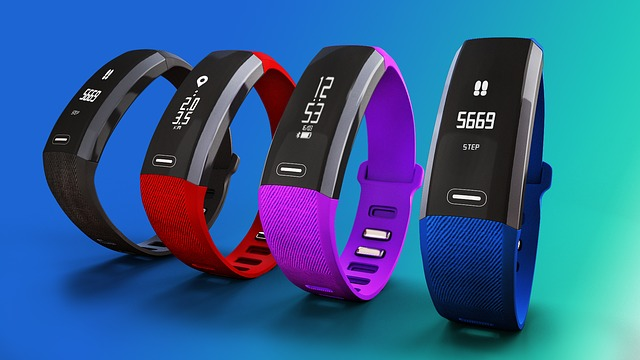
\includegraphics[width=\textwidth]{img/heart-rate-monitoring-device-1903997_640}

            \column[b]{.33\textwidth}
            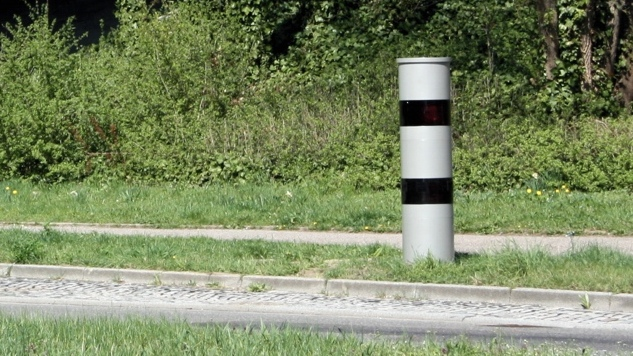
\includegraphics[width=\textwidth]{img/blitzer_pulverhausstrasse}

            \column[b]{.33\textwidth}
            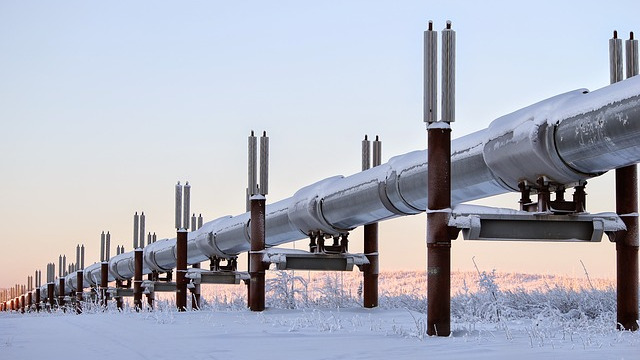
\includegraphics[width=\textwidth]{img/winter-681175_640}
        \end{columns}
    \end{block}
\end{frame}
}

%%% Folie
\begin{frame}{Eingebettete Systeme im Alltag}
    \begin{columns}
        \column{\dimexpr\paperwidth}
        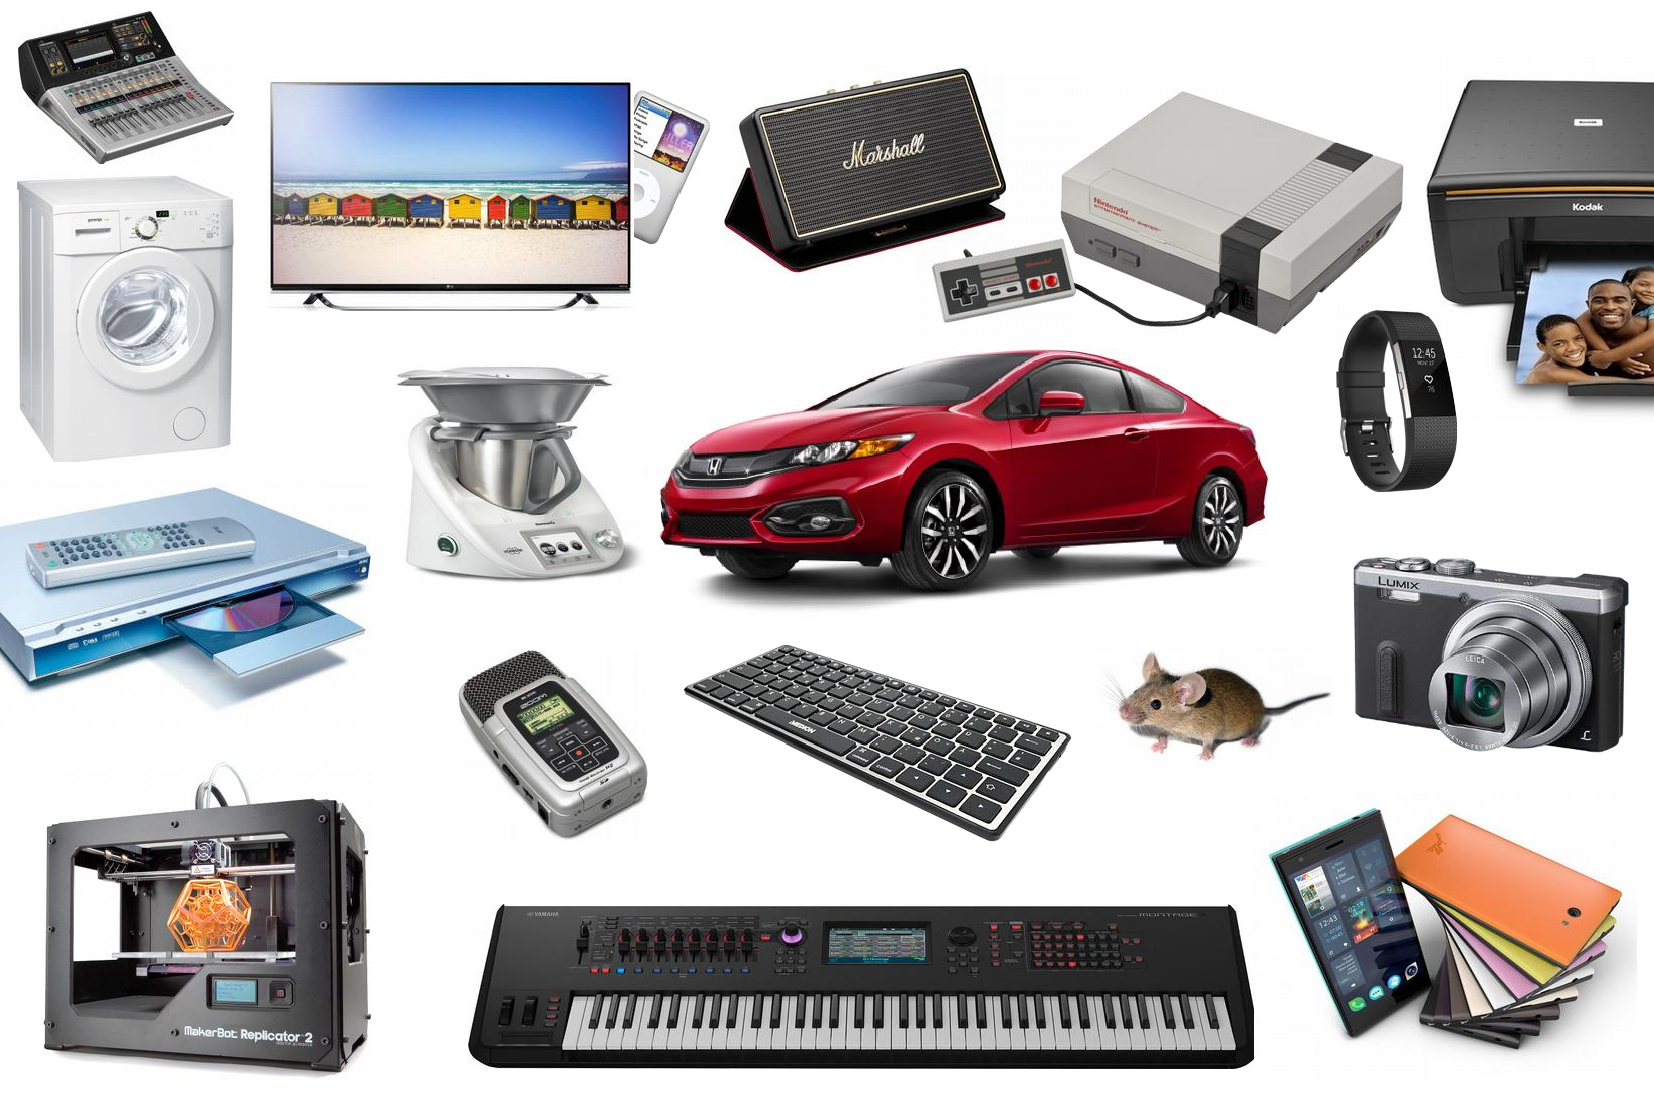
\includegraphics[width=\textwidth, height=\textheight-3em]{img/embedded_devices}
    \end{columns}
\end{frame}

%%% Folie
\begin{frame}{IoT-Devices im Alltag}
    \begin{columns}
        \begin{column}[b]{.45\textwidth}
            \begin{center}
                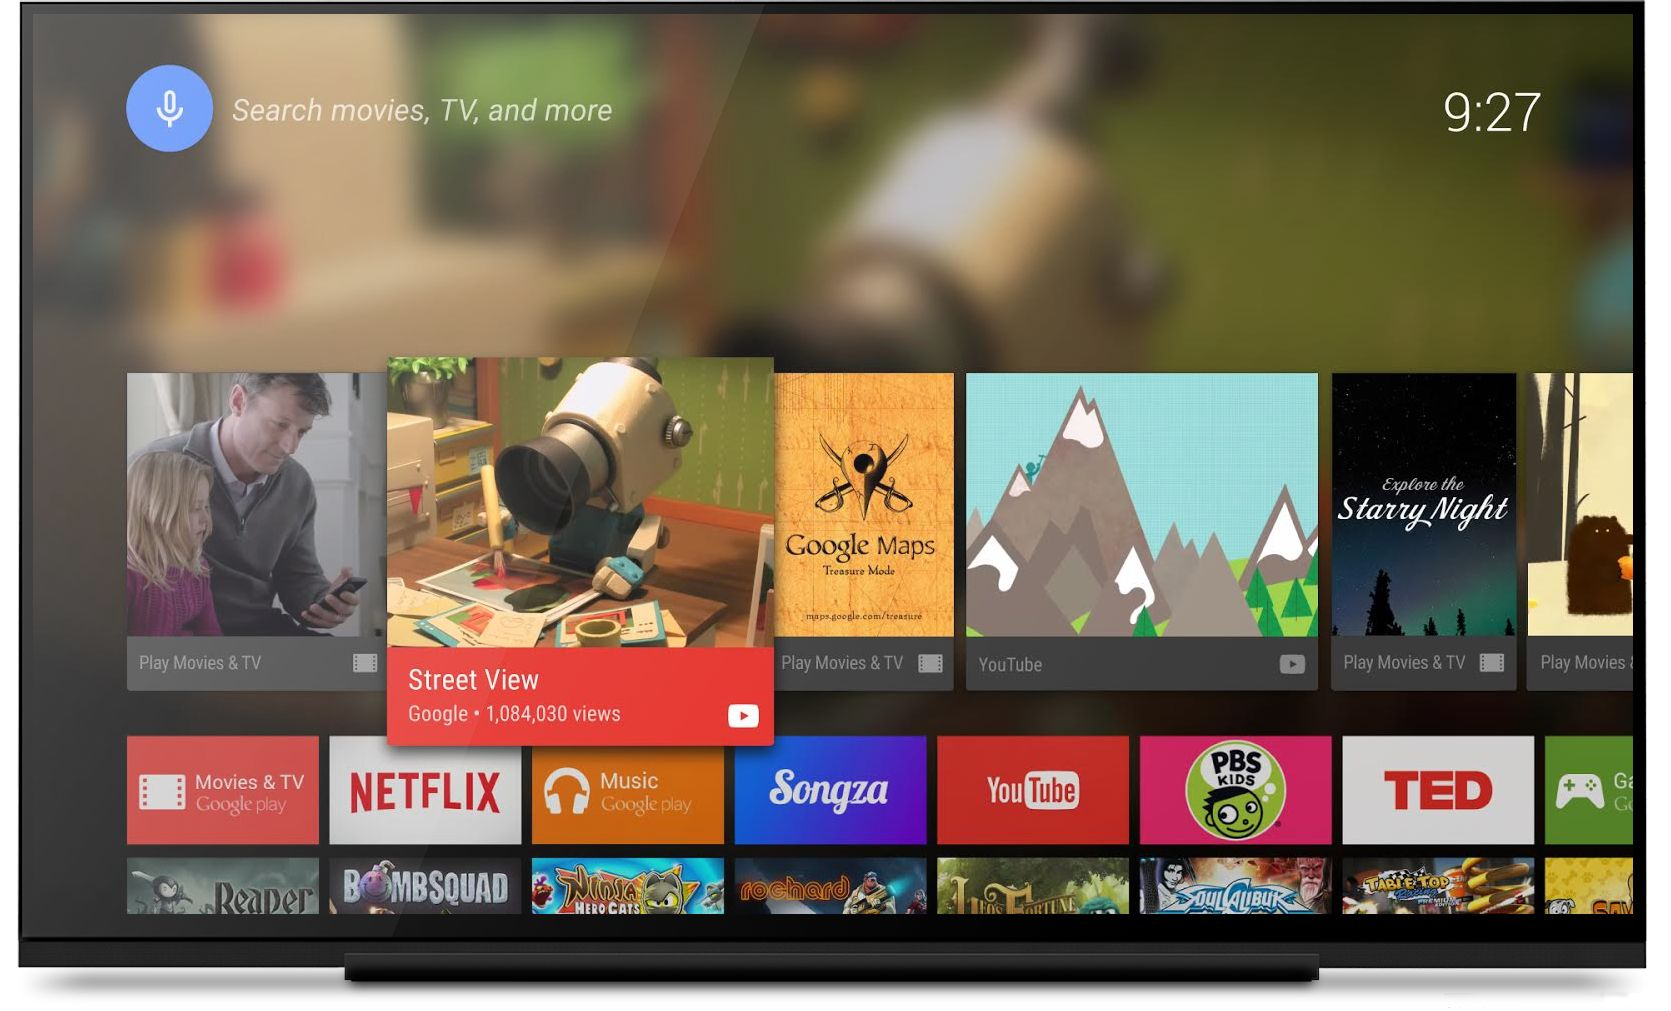
\includegraphics[width=\textwidth]{img/android_tv}
            \end{center}
        \end{column}
        \begin{column}[b]{.45\textwidth}
            \begin{center}
                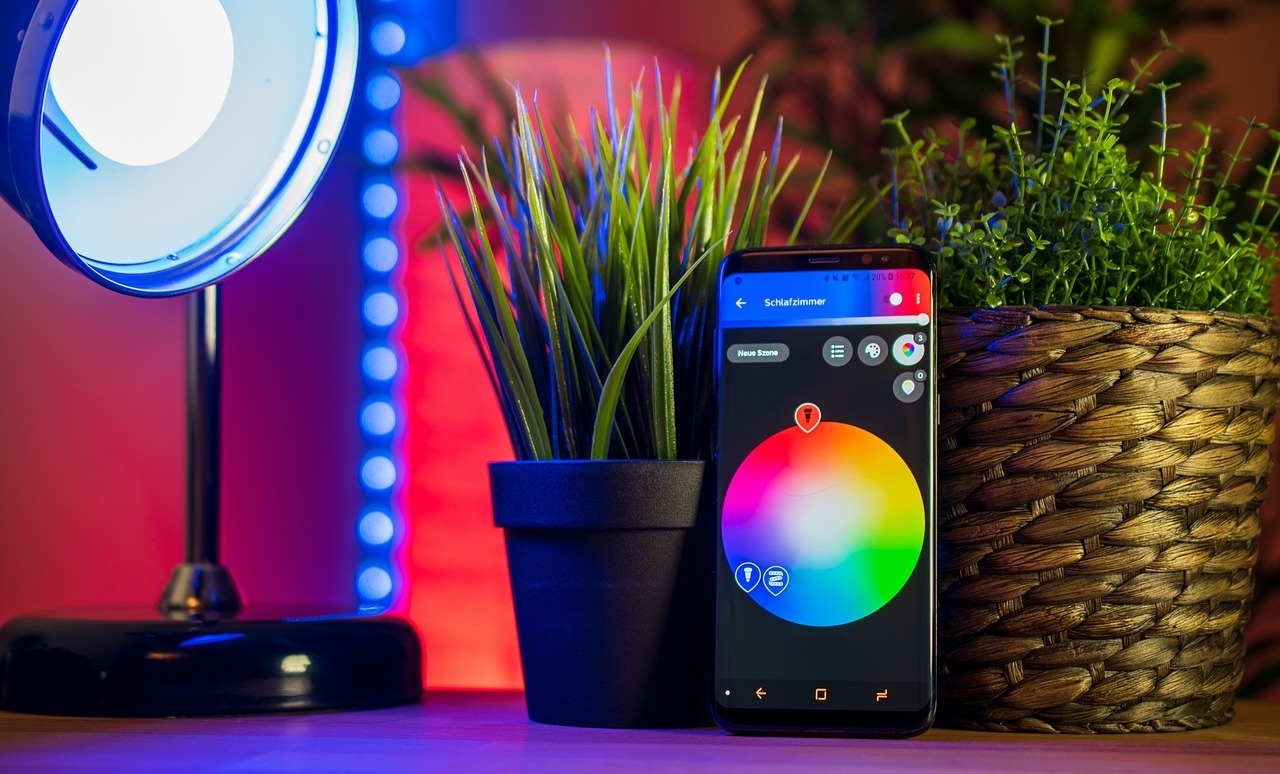
\includegraphics[width=\textwidth]{img/smart-home-3779361_1280}
            \end{center}
        \end{column}
    \end{columns}

    \begin{columns}
        \begin{column}[b]{.45\textwidth}
            \begin{center}
                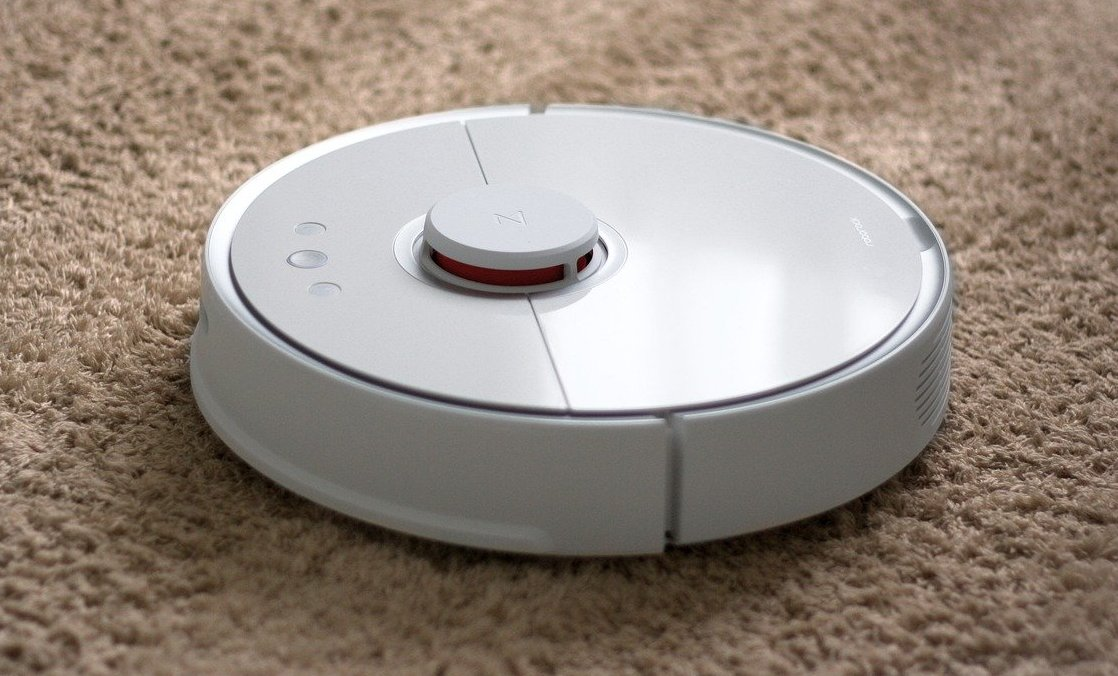
\includegraphics[width=\textwidth]{img/saugroboter}
            \end{center}
        \end{column}
        \begin{column}[b]{.45\textwidth}
            \begin{center}
                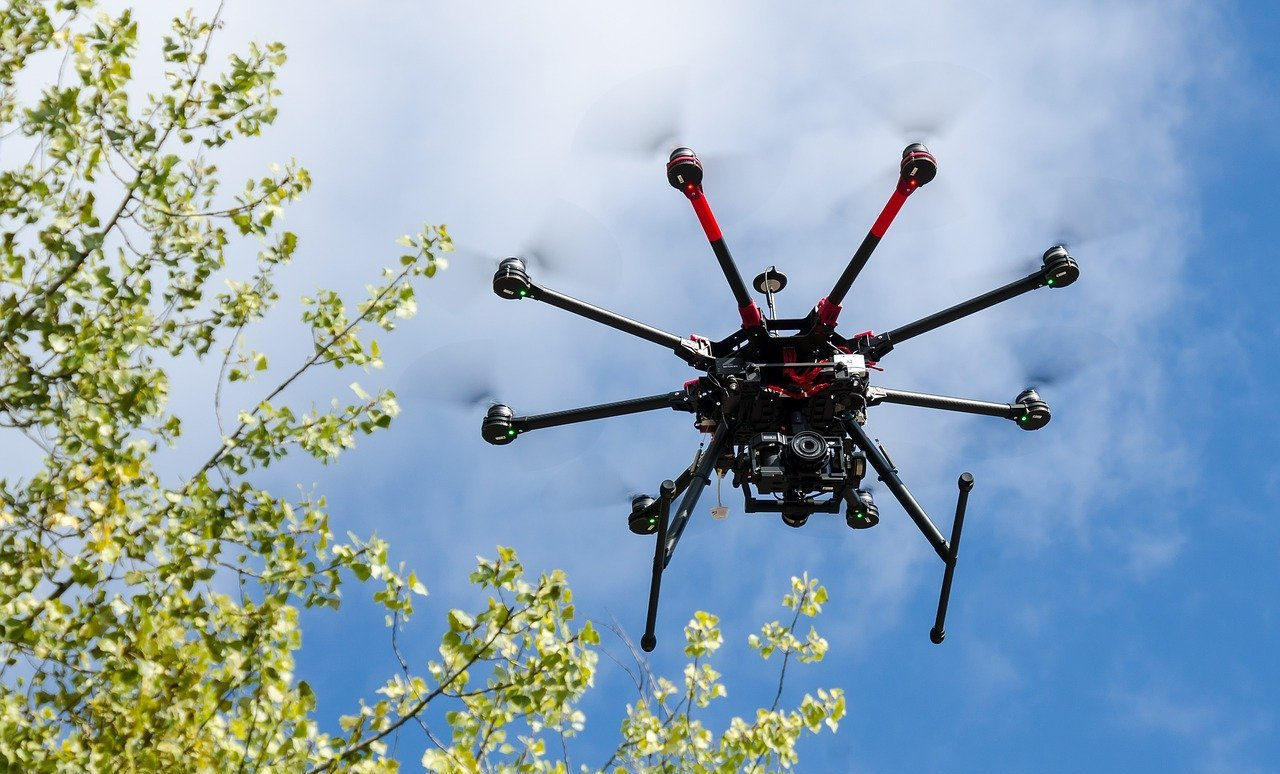
\includegraphics[width=\textwidth]{img/drone}
            \end{center}
        \end{column}
    \end{columns}
\end{frame}

%%% Folie
\begin{frame}{Industrielle IoT-Anwendungsfälle}
    \begin{columns}
        \begin{column}[b]{.45\textwidth}
            \begin{center}
                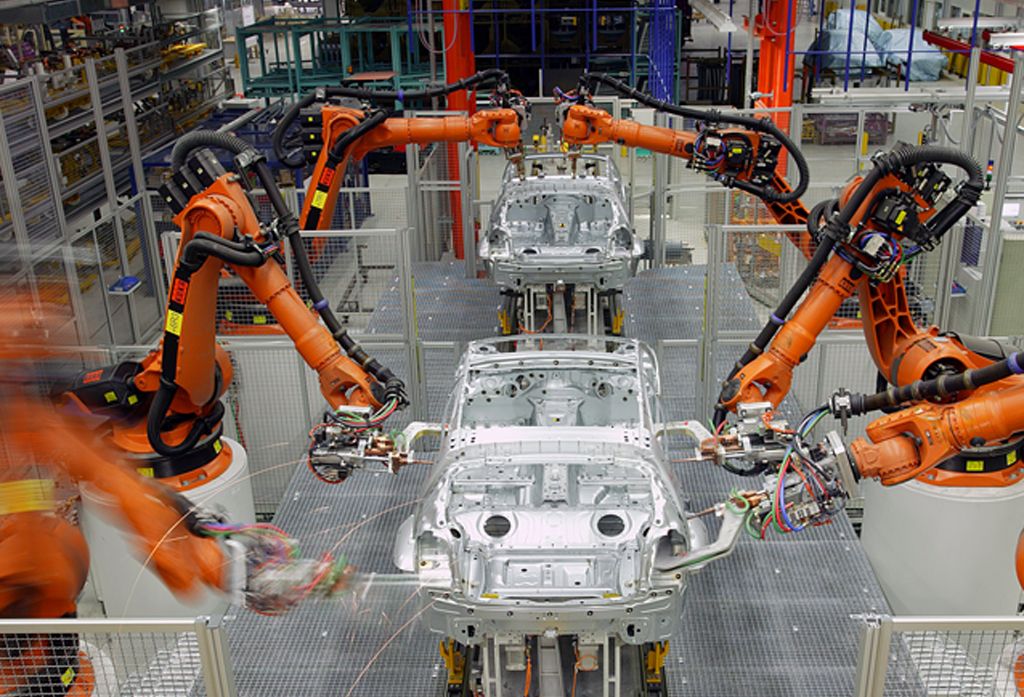
\includegraphics[width=\textwidth]{img/iiot-fertigung}
            \end{center}
        \end{column}
        \begin{column}[b]{.45\textwidth}
            \begin{center}
                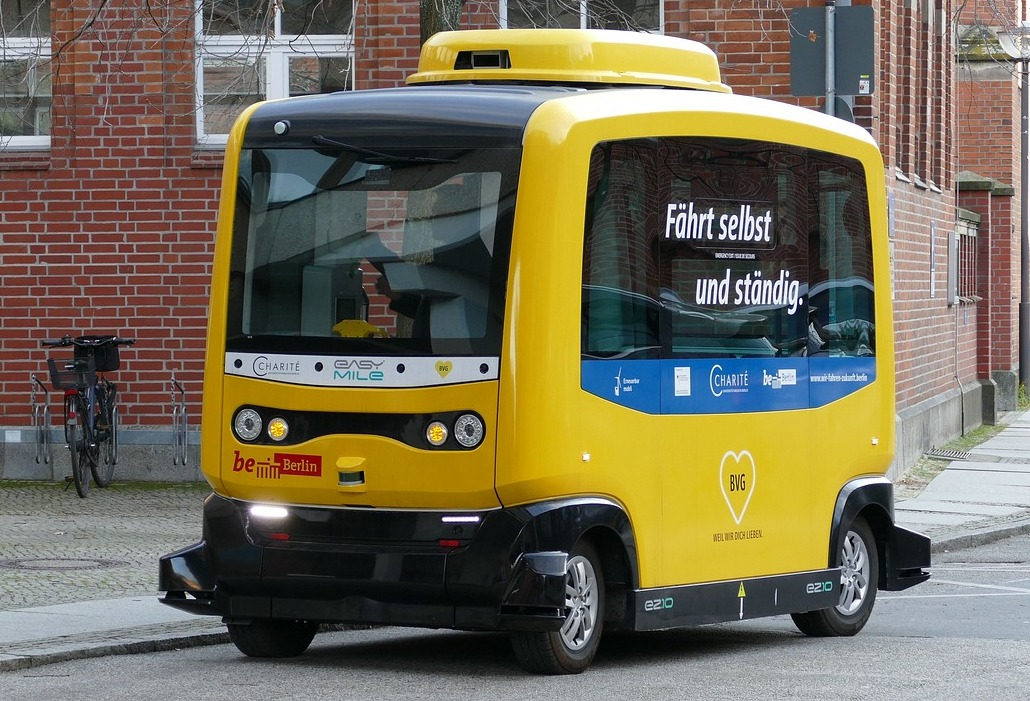
\includegraphics[width=\textwidth]{img/iiot-autonomes-fahren}
            \end{center}
        \end{column}
    \end{columns}

    \begin{columns}
        \begin{column}[b]{.45\textwidth}
            \begin{center}
                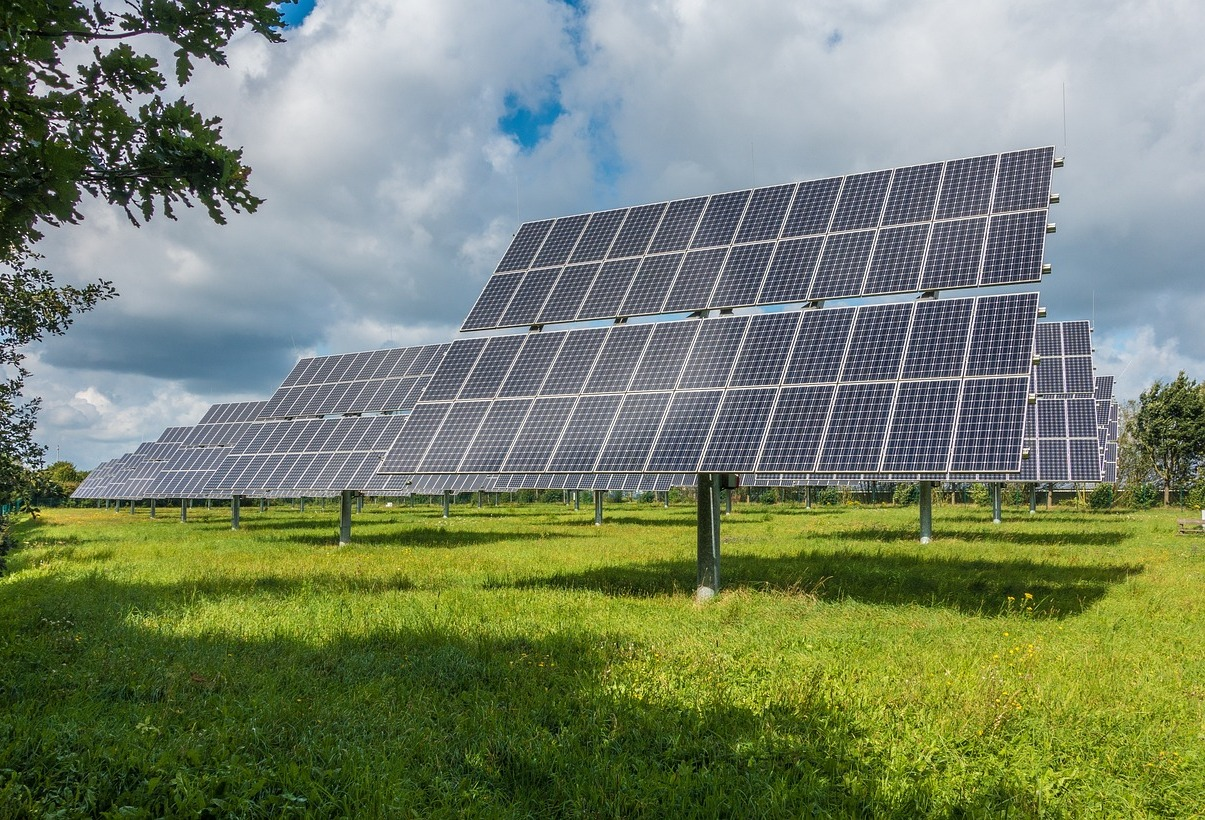
\includegraphics[width=\textwidth]{img/iiot-energie}
            \end{center}
        \end{column}
        \begin{column}[b]{.45\textwidth}
            \begin{center}
                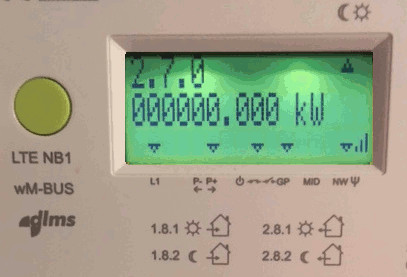
\includegraphics[width=\textwidth]{img/iiot-smartmeter}
            \end{center}
        \end{column}
    \end{columns}
\end{frame}

%-------------------------------------------------------------------------------
\section{Technische Grundlagen}
%-------------------------------------------------------------------------------

%%% Folie
{
\setbeamertemplate{background canvas}{
    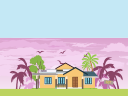
\includegraphics[height=\paperheight, width=\paperwidth]{img/themengebiete1}
}

\begin{frame}[fragile]{IoT -- Ein Haus mit tiefem Keller}
    \only<beamer:2|handout:0>{
        \transdissolve

        \begin{tikzpicture}[remember picture,overlay]
            \node at (5.4cm,0.2cm){
                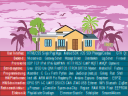
\includegraphics[height=\paperheight, width=\paperwidth]{img/themengebiete2}
            };
        \end{tikzpicture}
    }
\end{frame}
}

{
\setbeamertemplate{background canvas}{
    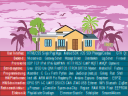
\includegraphics[height=\paperheight, width=\paperwidth]{img/themengebiete2}
}

\begin{frame}<handout>[plain]
\end{frame}
}

%%% Folie
\begin{frame}{Beispiel einer typischen IoT-Architektur}
    \begin{columns}
        \column{\dimexpr\paperwidth-10pt}
        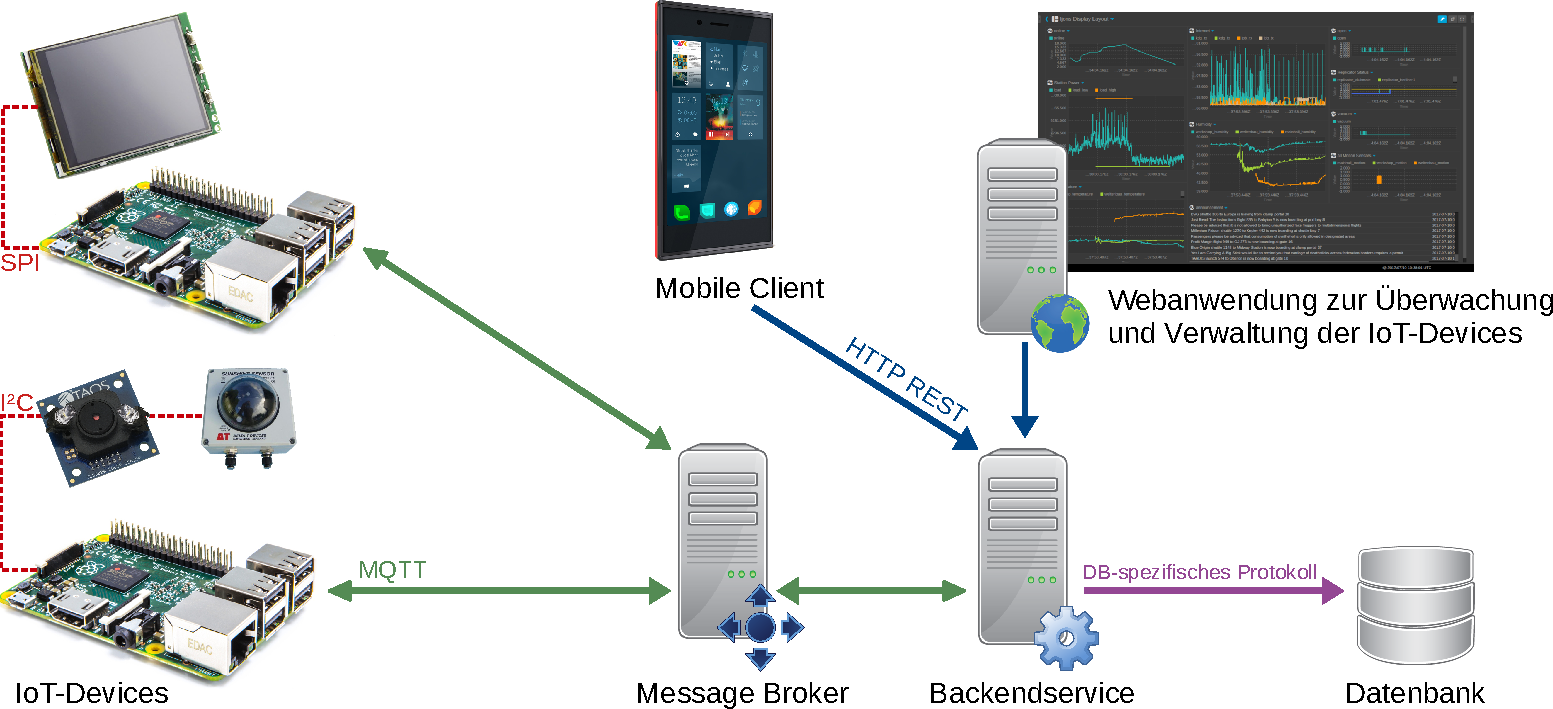
\includegraphics[width=\textwidth]{img/architektur_beispiel}
    \end{columns}
\end{frame}

%%% Folie
{
\setbeamertemplate{background canvas}{
    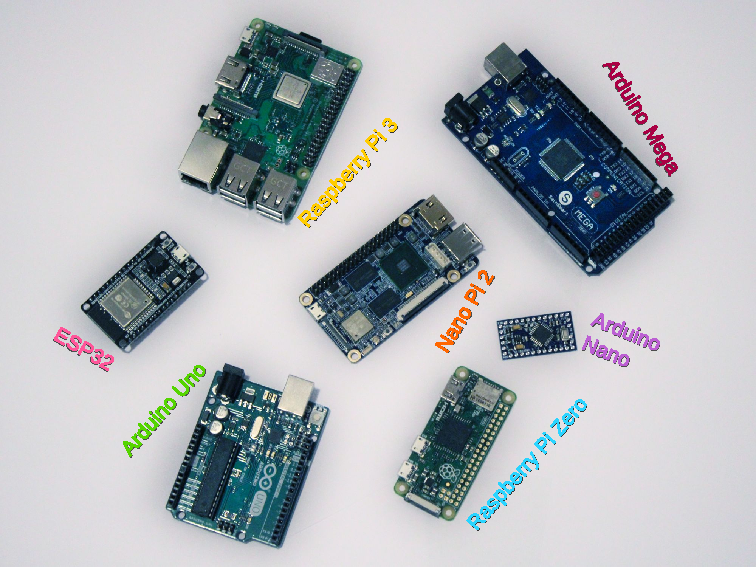
\includegraphics[height=\paperheight, width=\paperwidth]{img/sbc_auswahl}
}

\begin{frame}[plain]
\end{frame}
}

%%% Folie
{
\scriptsize

\begin{frame}{Beispiele für typische Single Board Computer}
    \begin{columns}
        \begin{column}[b]{.5\textwidth}
            \textbf{Arduino Nano} \\
            \smallskip
            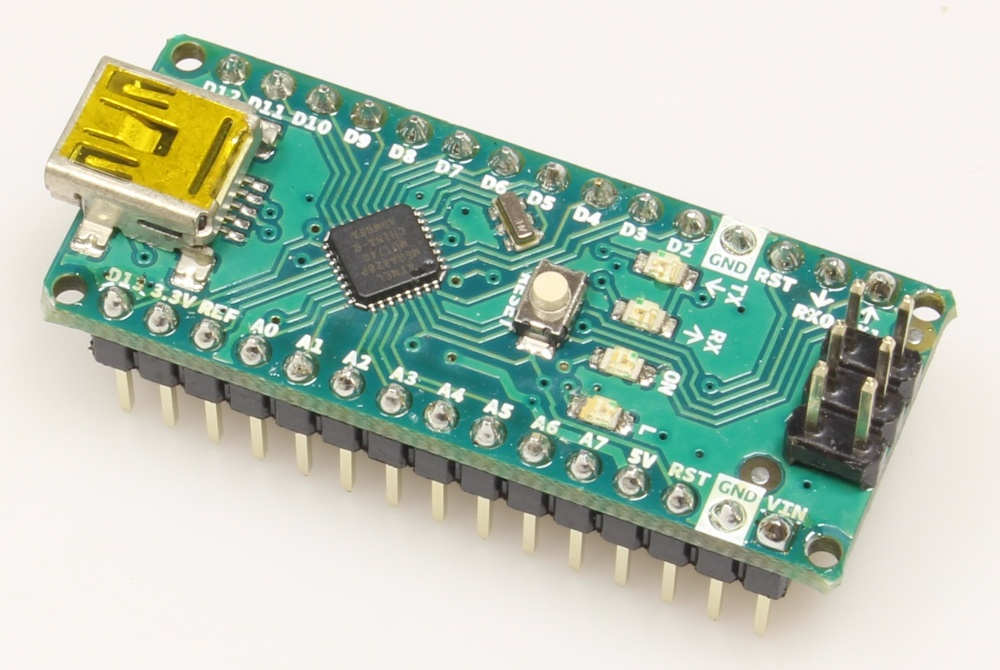
\includegraphics[width=.5\textwidth]{img/sbc-arduino_nano}

            \begin{itemize}
                \setlength{\itemindent}{-1em}
                \setlength\itemsep{0em}
                \item 16 MHz ATmega328 CPU
                \item 32 KiB Flash EEPROM, 2 KiB SRAM
                \item 22 $\times$ Digital-, 8 $\times$ Analog-, 6 $\times$ PWM-Ausgang
            \end{itemize}
        \end{column}

        \begin{column}[b]{.5\textwidth}
            \textbf{PyBoard} \\
            \smallskip
            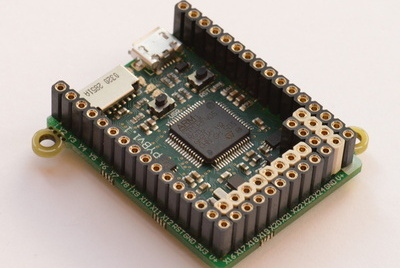
\includegraphics[width=.5\textwidth]{img/sbc-pyboard}

            \begin{itemize}
                \setlength{\itemindent}{-1em}
                \setlength\itemsep{0em}
                \item 168 MHz ARM Cortex M4 CPU
                \item 1024 KiB Flash ROM, 192 KiB RAM
                \item 29 GPIO, 3 $\times$ 12-bit ADC, 2 $\times$ 12-bit DAC
            \end{itemize}
        \end{column}
    \end{columns}

    \bigskip

    \begin{columns}
        \begin{column}[b]{.5\textwidth}
            \textbf{ESP32} \\
            \smallskip
            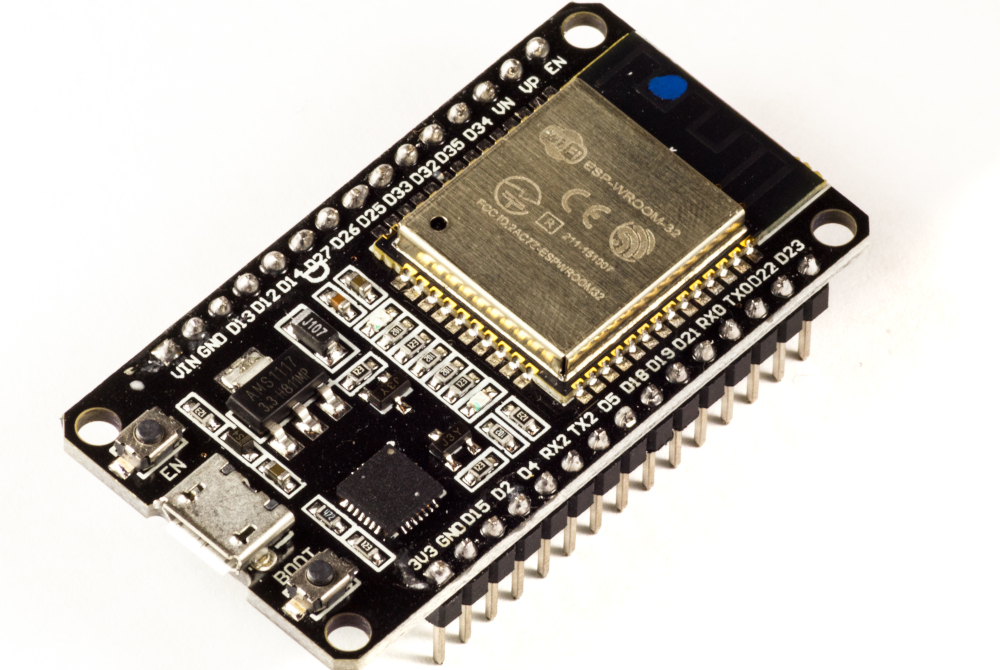
\includegraphics[width=.5\textwidth]{img/sbc-esp32}

            \begin{itemize}
                \setlength{\itemindent}{-1em}
                \setlength\itemsep{0em}
                \item 160 -- 240 MHz Xtensa LX6 Dual-Core CPU
                \item 2 $\times$ 160 KiB RAM (statisch/dynamisch)
                \item GPIO, WLAN, Bluetooth, ...
            \end{itemize}
        \end{column}

        \begin{column}[b]{.5\textwidth}
            \textbf{Raspberry Pi 4} \\
            \smallskip
            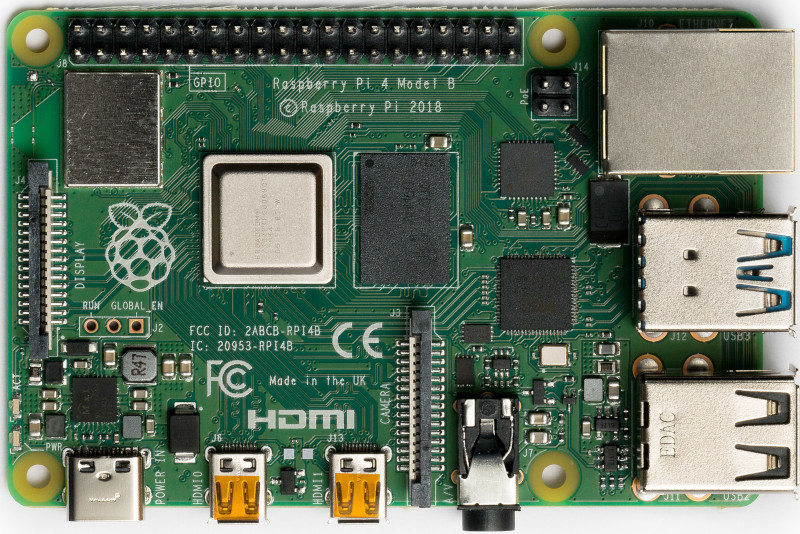
\includegraphics[width=.5\textwidth]{img/sbc-raspberrypi}

            \begin{itemize}
                \setlength{\itemindent}{-1em}
                \setlength\itemsep{0em}
                \item BCM2711 ARM v8 CPU, Quad Core
                \item 4 oder 8 GiB RAM
                \item GPIO, WLAN, Bluetooth, USB, HDMI, ...
            \end{itemize}
        \end{column}
    \end{columns}
\end{frame}
}

%%% Folie
{
\footnotesize

\begin{frame}{Typischer Systemaufbau eingebetteter Systeme}
    \begin{columns}
        \column{\dimexpr\paperwidth}
        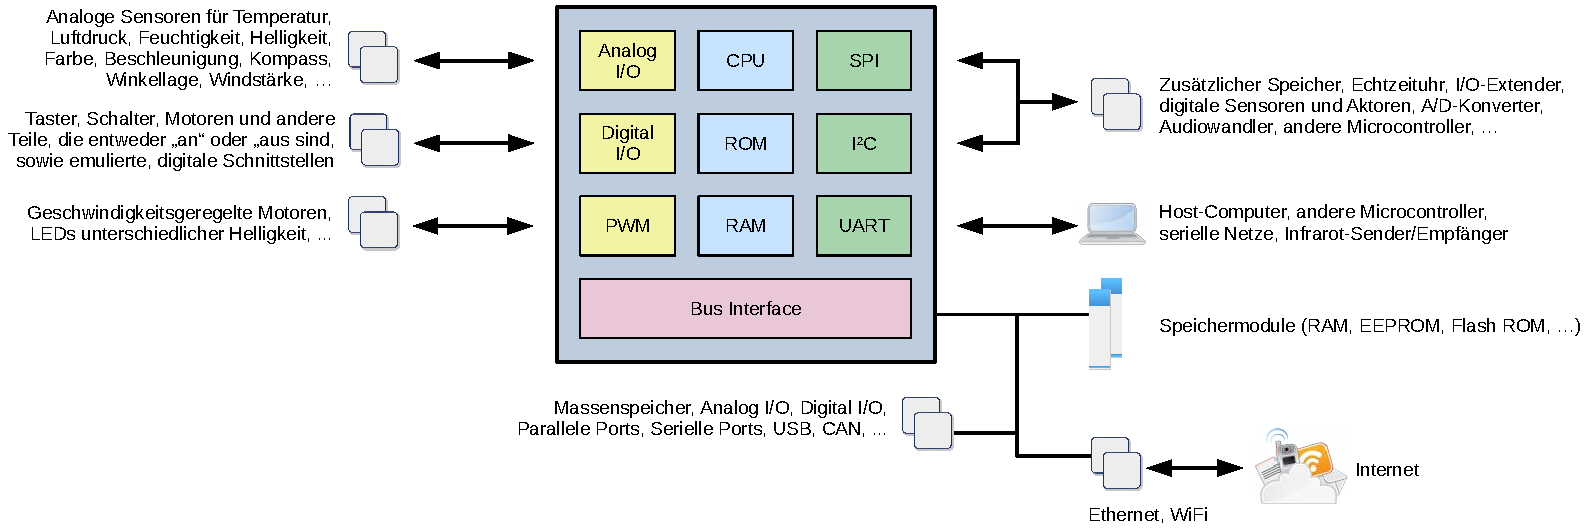
\includegraphics[width=\paperwidth]{img/mc_aufbau}
    \end{columns}

    \bigskip

    \begin{columns}
        \begin{column}[T]{.5\textwidth}
            \textbf{Durchschnittlicher Microcontroller}
            \begin{itemize}
                \item 16 MHz Taktgeschwindigkeit
                \item 8 Bit Wortbreite
                \item 32 kB Programmspeicher
                \item 2 kB Hauptspeicher
                \item 14 General Purpose I/Os
                \item Kein Betriebssystem
            \end{itemize}
        \end{column}
        \begin{column}[T]{.5\textwidth}
            \textbf{Durchschnittlicher System-on-a-Chip}
            \begin{itemize}
                \item $\geq$ 200 MHz Taktgeschwindigkeit
                \item $\geq$ 32 Bit Wortbreite
                \item $\geq$ 512 MB Flash ROM
                \item $\geq$ 16 MB Hauptspeicher
                \item $\geq$ 30 General Purpose I/Os
                \item Mit oder ohne Betriebssystem
            \end{itemize}
        \end{column}
    \end{columns}
\end{frame}
}

%%% Folie
{
\scriptsize

\begin{frame}{Mikroprozessoren für eingebettete Systeme}
    \begin{columns}
        \column{.2\textwidth}
        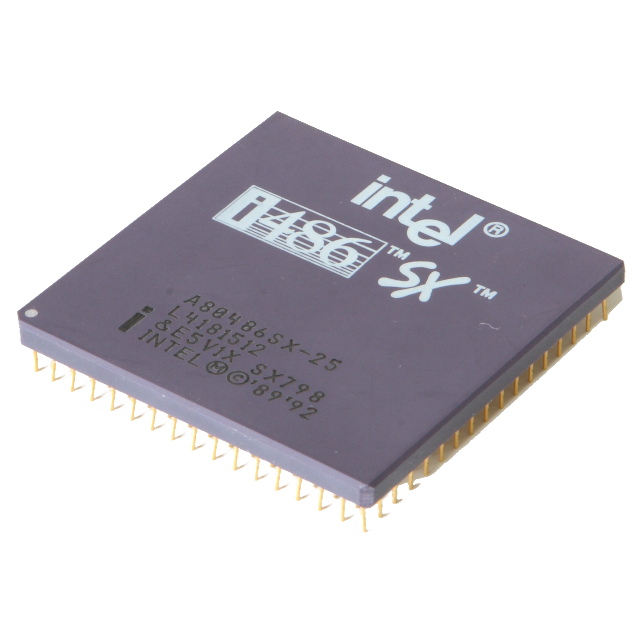
\includegraphics[width=.9\linewidth]{img/chip-intel-486}

        \column{.8\textwidth}
        \begin{block}{Diskreter Hauptprozessor}
            \Justified{
                \smallskip

                Bildet das Herzstück eines jeden Computers bzw. stellt den Computer
                im engeren Sinne dar, basierend auf dem Prinzip
                \textbf{Eingabe-Verarbeitung-Ausgabe}. Kommuniziert daher über eine
                \textbf{Speicherschnittstelle} bestehend aus Adress-, Daten- und Steuerleitungen
                mit externen Speicher- und I/O-Bausteinen.
            }

            \smallskip

            \textbf{Beispiele}: Intel 8051, MOS 6502, Motorola 68000, …
        \end{block}
    \end{columns}

    \begin{columns}
        \column{.2\textwidth}
        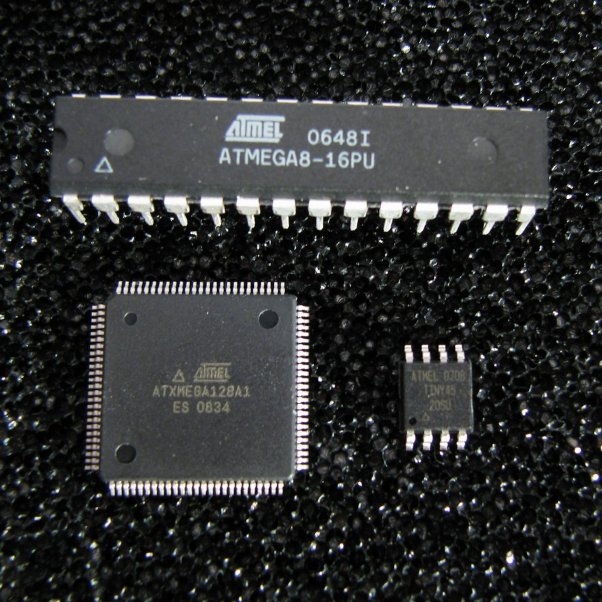
\includegraphics[width=.9\linewidth]{img/chip-avr-atmega}

        \column{.8\textwidth}
        \begin{block}{Microcontroller}
            \Justified{
                \smallskip

                Integriert eine einfache CPU (oftmals mit nur 8-bit Datenbreite)
                sowie RAM und ROM auf einem Chip, um ein kleines Programm zur
                Steuerung mit externer Peripherie auszuführen. Bietet meist keine
                externe Speicherschnittstelle, dafür aber I/O-Möglichkeiten wie
                \textbf{GPIO}, \textbf{Serielle Schnittstellen}, \textbf{A/D-Wandler}
                uwm.
            }

            \smallskip

            \textbf{Beispiele}: AVR ATtiny, AVR ATmega, PIC, ARM STM32F722, …
        \end{block}
    \end{columns}

    \begin{columns}
        \column{.2\textwidth}
        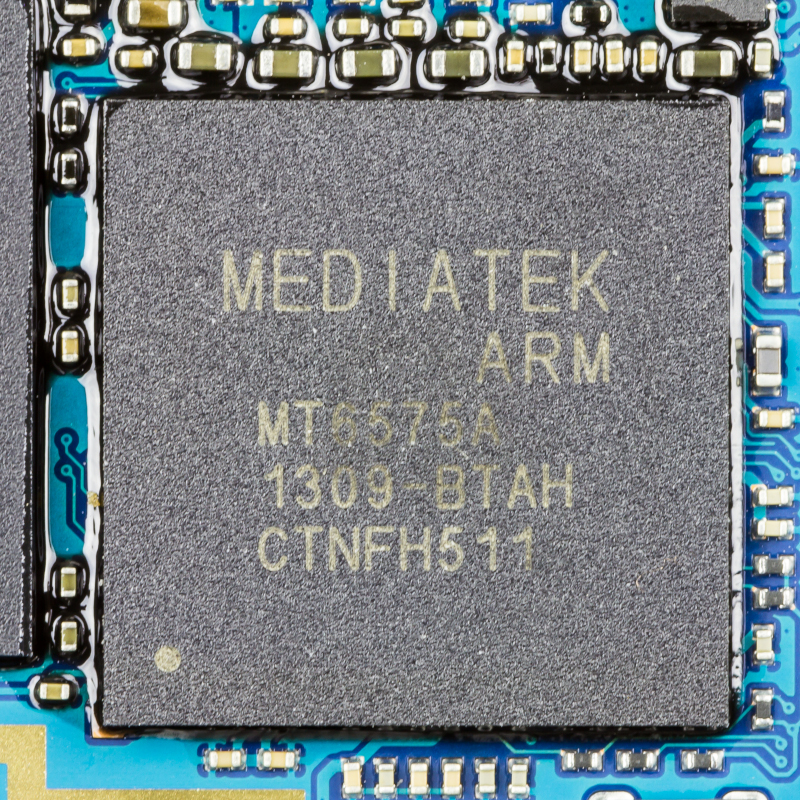
\includegraphics[width=.9\linewidth]{img/chip-arm-cortex}

        \column{.8\textwidth}
        \begin{block}{System-on-a-Chip}
            \Justified{
                \smallskip

                Wie ein Microcontroller nur mit einem \textbf{viel leistungsstärkeren
                Rechenkern}, dessen Performance mit dedizierten CPUs vergleichbar ist.
                \textbf{Externer RAM und ROM} werden wie bei einer diskreten CPU über
                ein Speicherinterface angebunden. Darüber hinaus werden oft auch
                \textbf{komplexe Komponenten} wie GPUs, WiFi, Bluetooth, HDMI, etc.
                auf demselben Chip untergebracht.
            }

            \smallskip

            \textbf{Beispiele}: ARM Cortex, AMD AU1000, …
        \end{block}
    \end{columns}
\end{frame}
}

%%% Folie
{
\scriptsize

\begin{frame}{Fallbeispiel: Die erste Mondlandung}
    \begin{columns}
        \column{\dimexpr\paperwidth}
        \vskip -.8em
        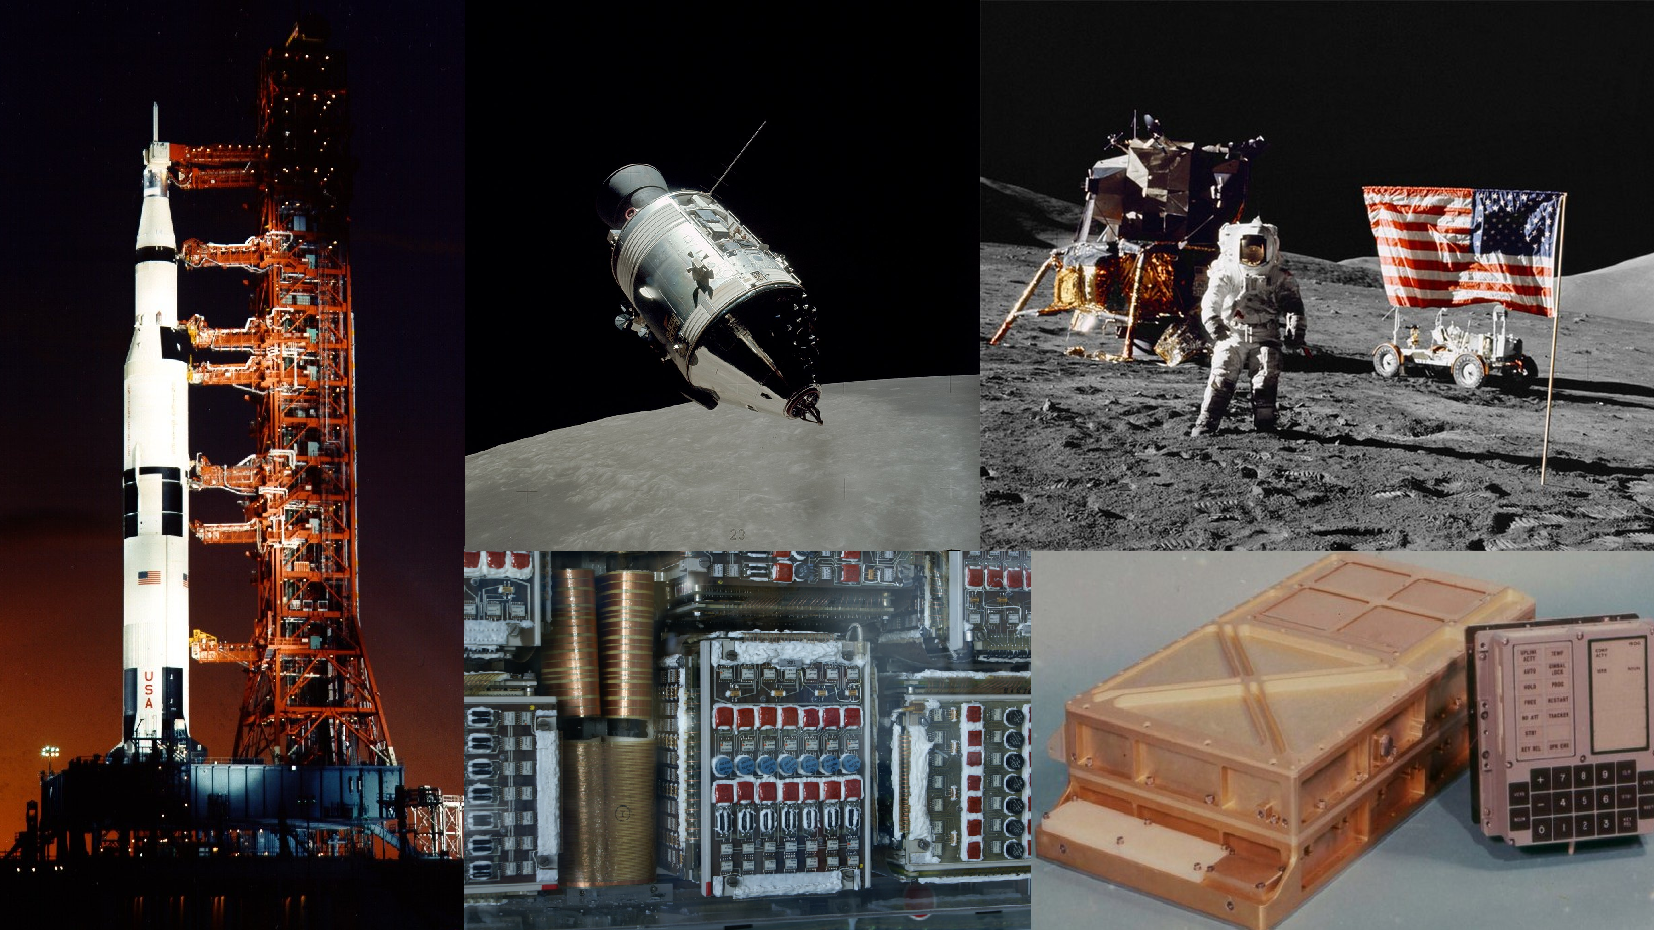
\includegraphics[width=\textwidth]{img/apollo}
    \end{columns}

    \vskip .5em

    \begin{columns}
        \column{\dimexpr\paperwidth-2em}
        \Justified{
            \textbf{21. Juli 1969}: Apollo 11 bringt die ersten Menschen zum Mond und
            wieder zur Erde zurück. Möglich wird dies unter Anderem durch den ,,Launch
            Vehicle Digital Computer'' der Saturn\,V Rakete und den ,,Apollo Guidance
            Computer'' in der Kommandokapsel.
        }
    \end{columns}
\end{frame}
}

%%% Folie
\begin{frame}[allowframebreaks]{Fallbeispiel: Diskret aufgebaute Rechnerarchitektur}
    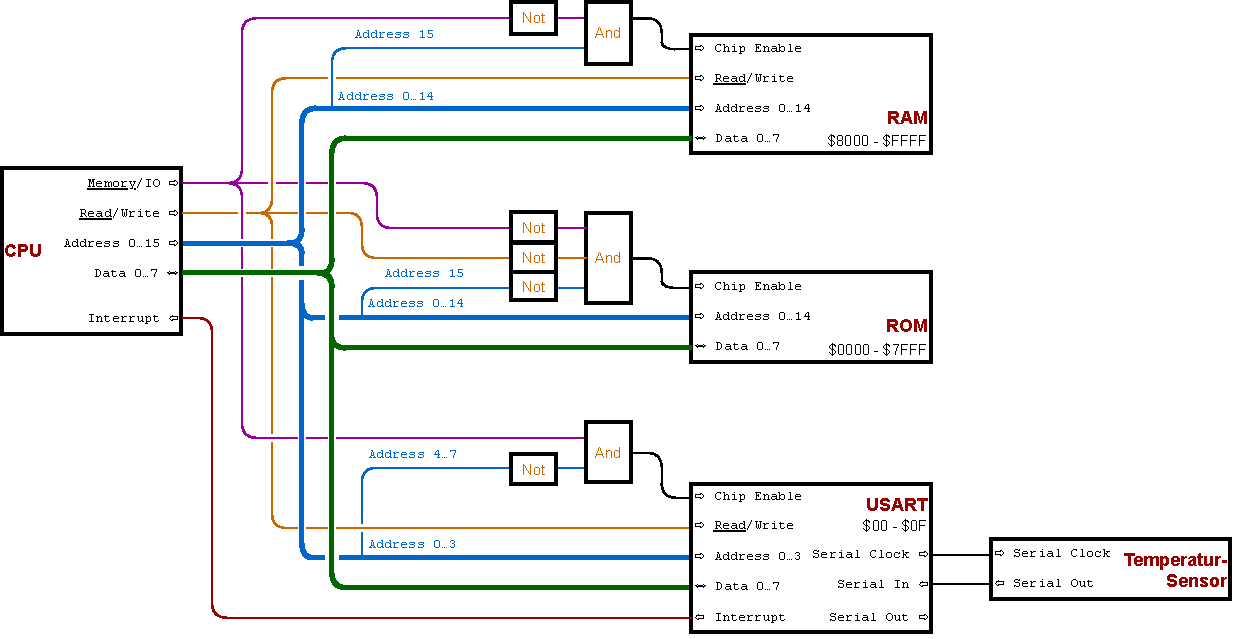
\includegraphics[width=\textwidth]{img/fallbeispiel-rechnerarchitektur}
    \bigskip

    \Justified{
        \footnotesize
        Vor der breiten Verfügbarkeit von Microcontrollern wurden selbst eingebettete
        Systeme mit diskreten Einzelbausteinen aufgebaut. In der Schemaskizze befinden
        sich daher integrierte Bausteine für den Hauptprozessor, Speicher, Ein- und
        Ausgabe sowie die Adresskodierung.
    }

    \framebreak

    \begin{center}
        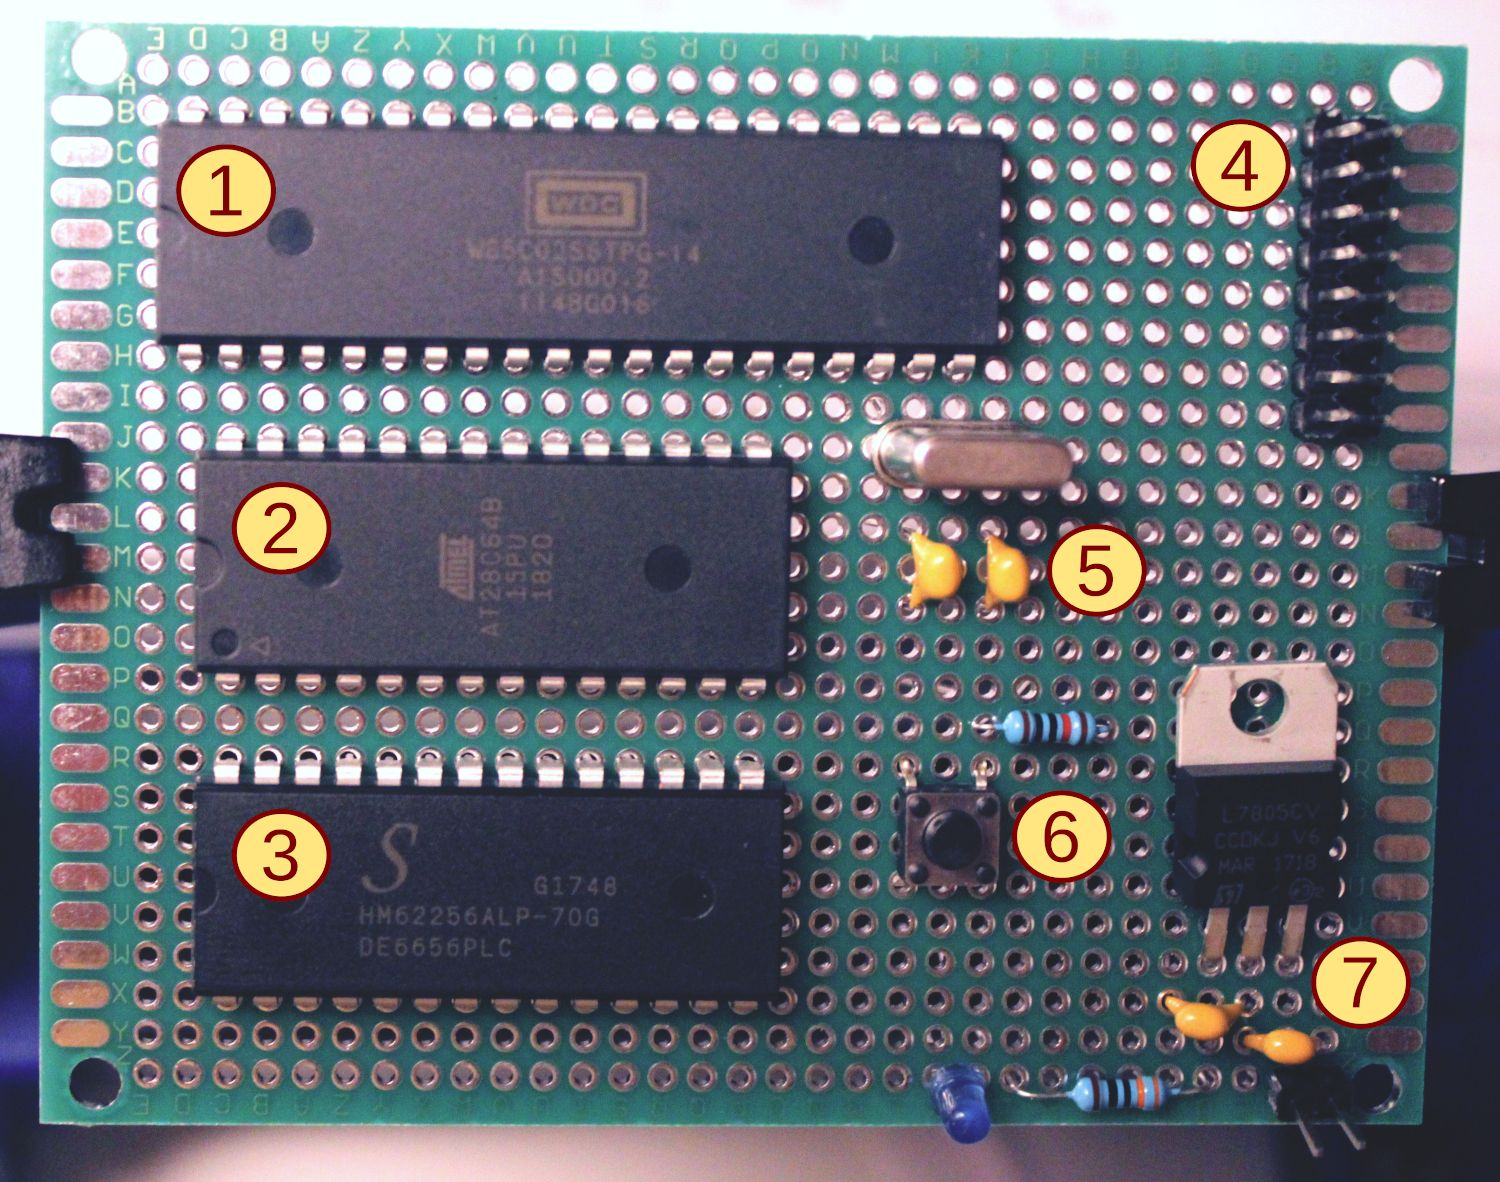
\includegraphics[height=0.5\textheight]{img/sbc_microprozessor2_klein}
    \end{center}

    \medskip

    \begin{columns}
        \begin{column}[T]{.5\textwidth}
            \textbf{Digitale Bausteine}
            \begin{enumerate}
                \item Mikroprozessor
                \item Programmspeicher
                \item Hauptspeicher
                \item I/O-Ports
            \end{enumerate}
        \end{column}
        \begin{column}[T]{.5\textwidth}
            \textbf{Hilfsschaltungen}
            \begin{enumerate}
                \setcounter{enumi}{4}
                \item Taktgeber
                \item Resetschalter
                \item Stromversorgung
                \item Adressdekodierung
            \end{enumerate}
        \end{column}
    \end{columns}
\end{frame}

%%% Folie
\begin{frame}[allowframebreaks]{Fallbeispiel: Yamaha SPX90 (1985)}
    \begin{center}
        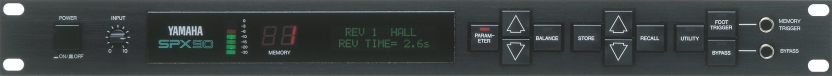
\includegraphics[width=\textwidth]{img/spx90-foto}
    \end{center}

    \smallskip

    \begin{itemize}
        \item Frühes, digitales Audio-Effektgerät für professionelle Anwendungen
        \item Hardwareaufbau zweigeteilt in eine Analog- und eine Digitalsektion
        \item \textbf{Analogsektion:} A/D-Wandlung und D/A-Wandlung der Audiosignale
        \item \textbf{Digitalsektion:} Diskret aufgebautes, eingebettetes Computersystem
    \end{itemize}

    \smallskip

    \begin{columns}
        \column[b]{.5\textwidth}
        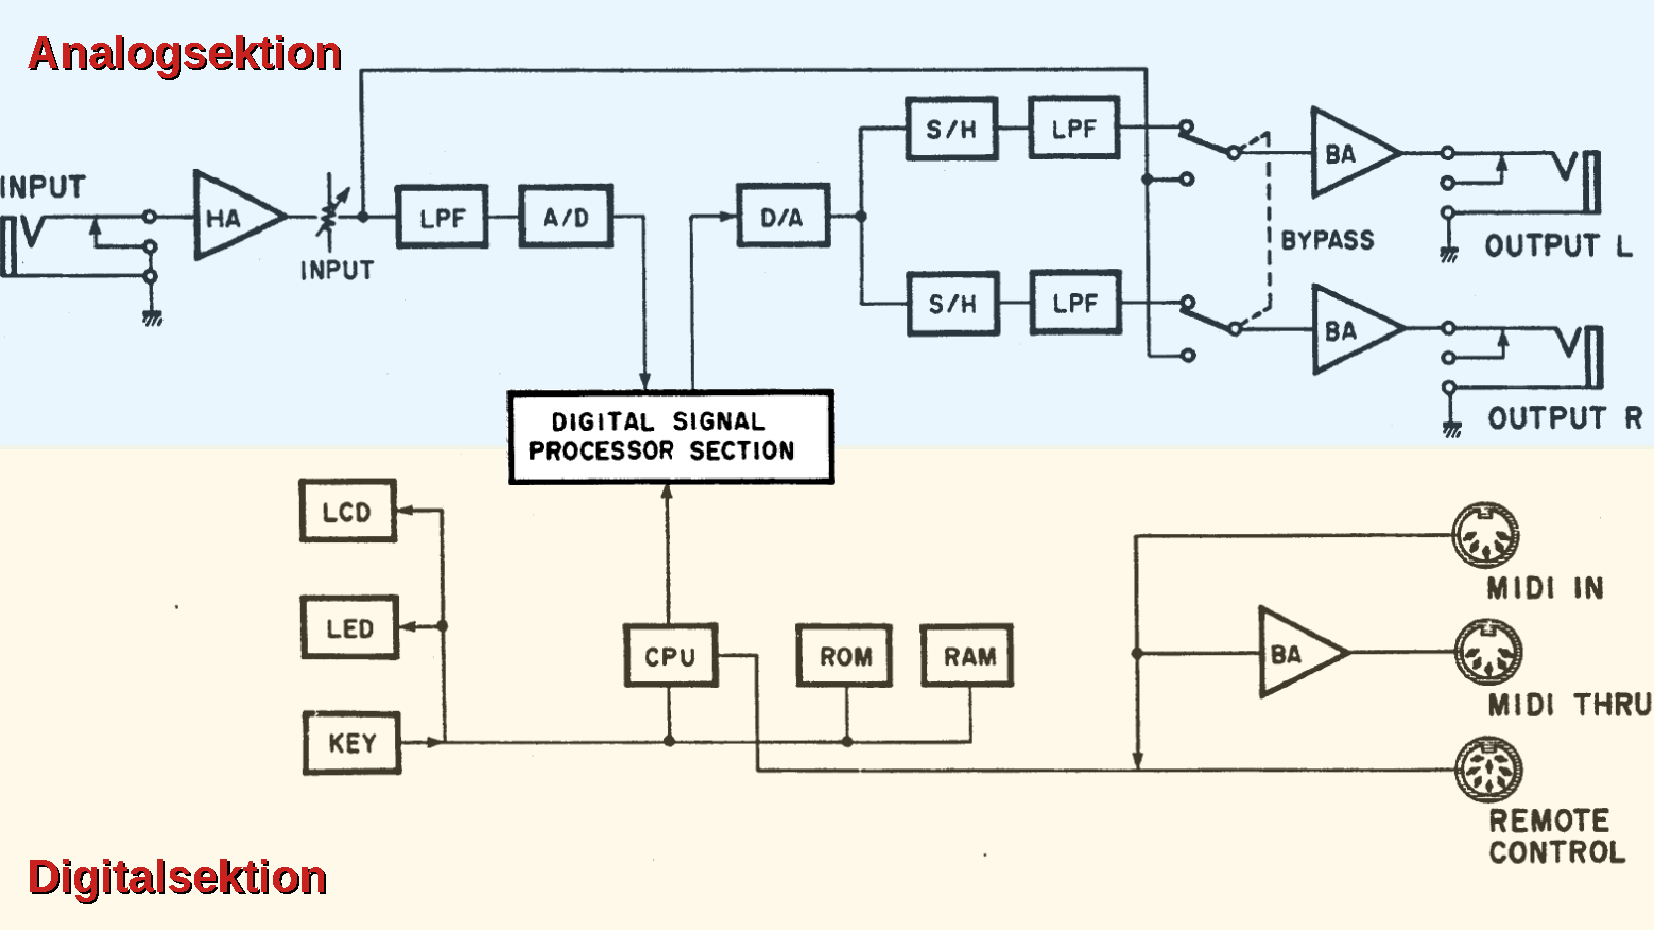
\includegraphics[width=\textwidth]{img/spx90-schaltplan-1}

        \column[b]{.5\textwidth}
        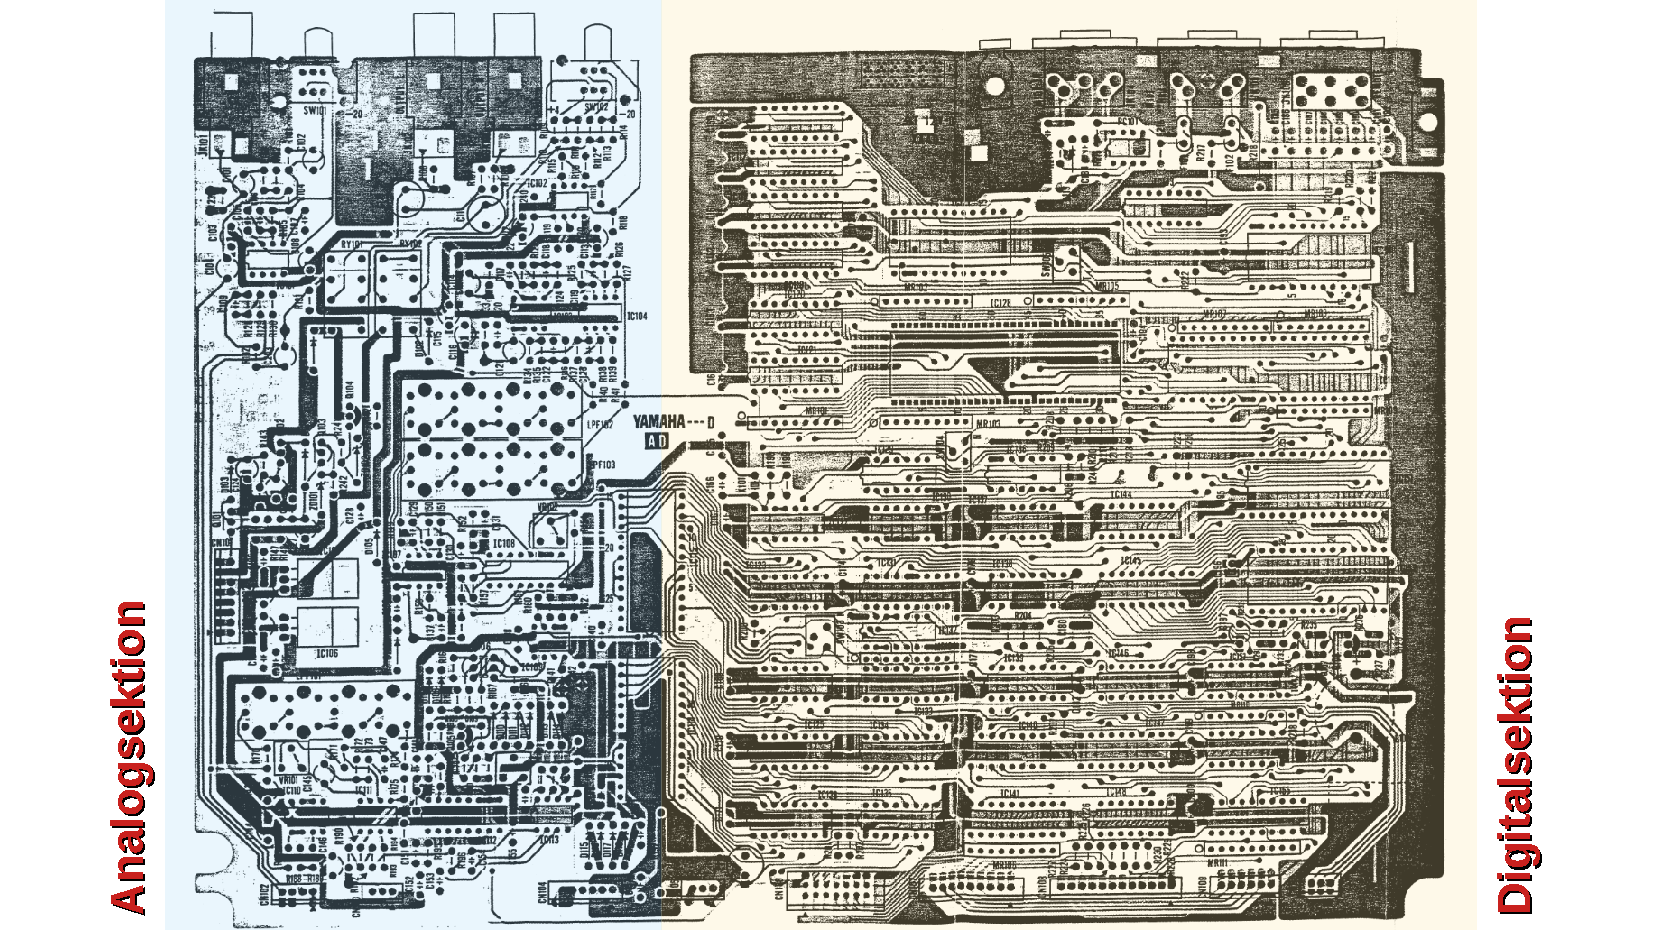
\includegraphics[width=\textwidth]{img/spx90-schaltplan-2}
    \end{columns}

    \bigskip

    \begin{columns}
        \column{\dimexpr\paperwidth}
        \vskip -.35em
        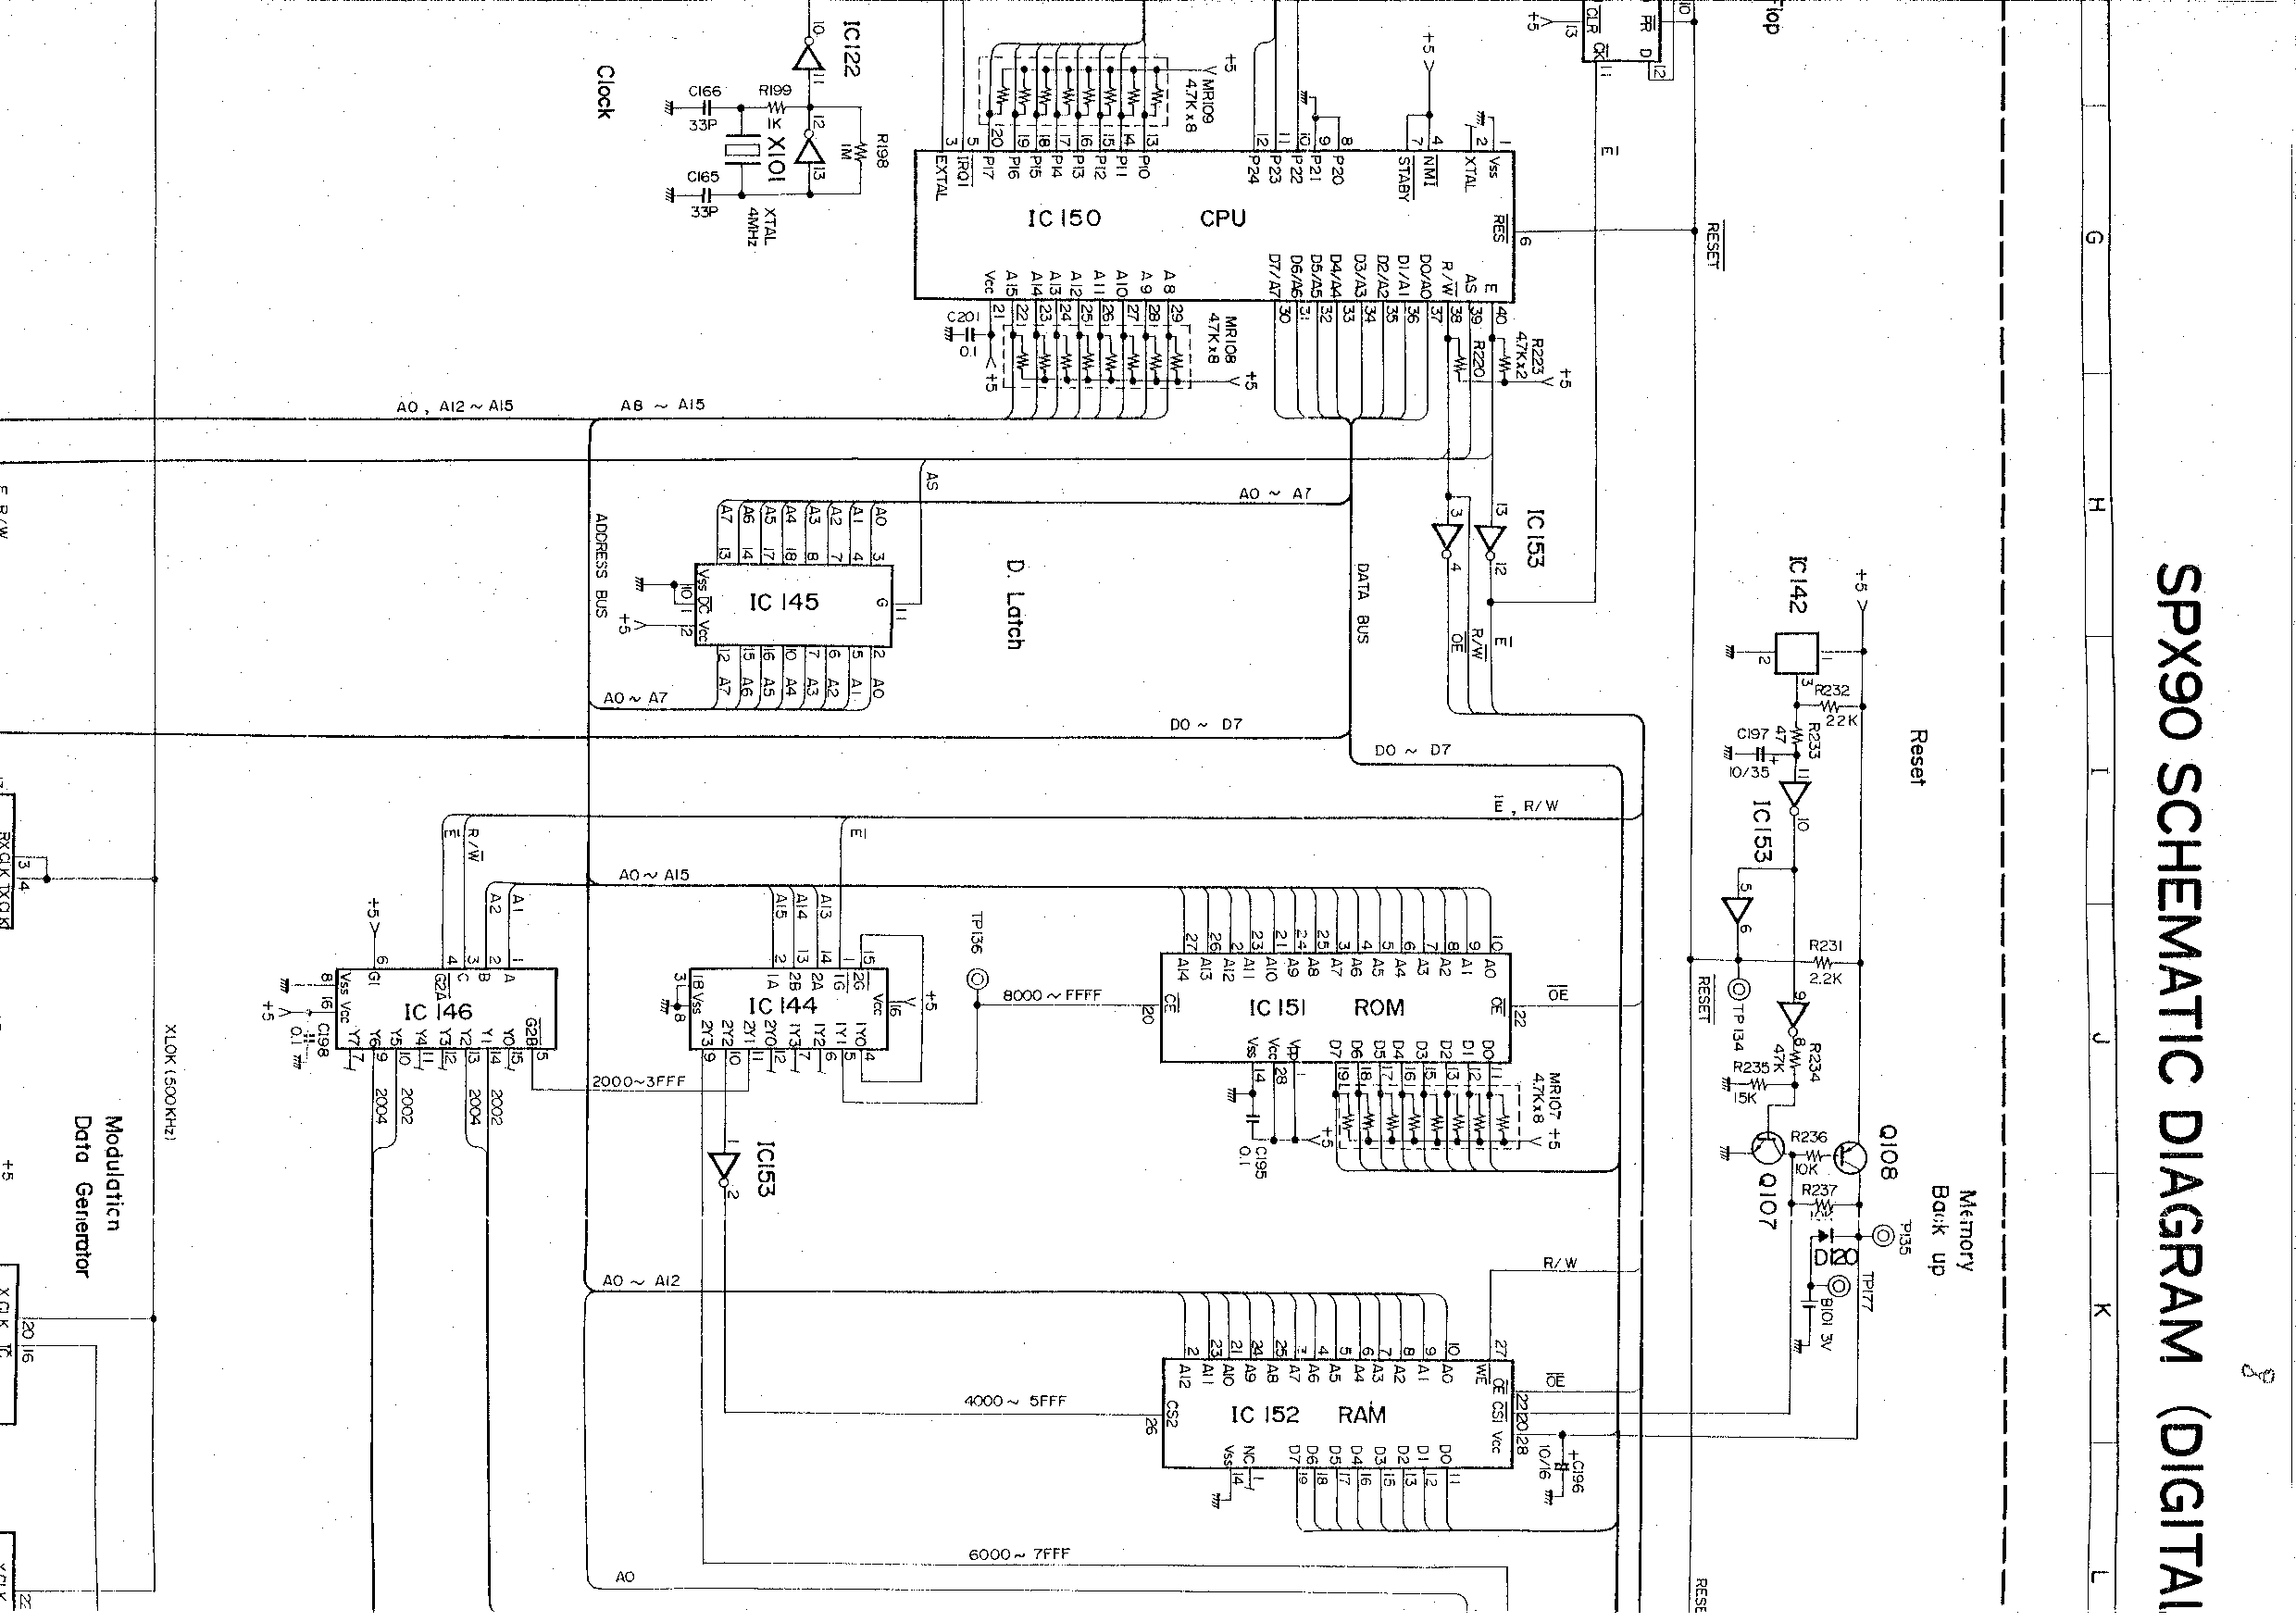
\includegraphics[width=\textwidth]{img/spx90-cpuboard}
    \end{columns}

\end{frame}

%%% Folie
{
\scriptsize

\begin{frame}{Fallbeispiel: LED-Laufschrift $\times$ 4}
    \begin{columns}
        \column{.5\textwidth}
        \textbf{Arduino Board}
        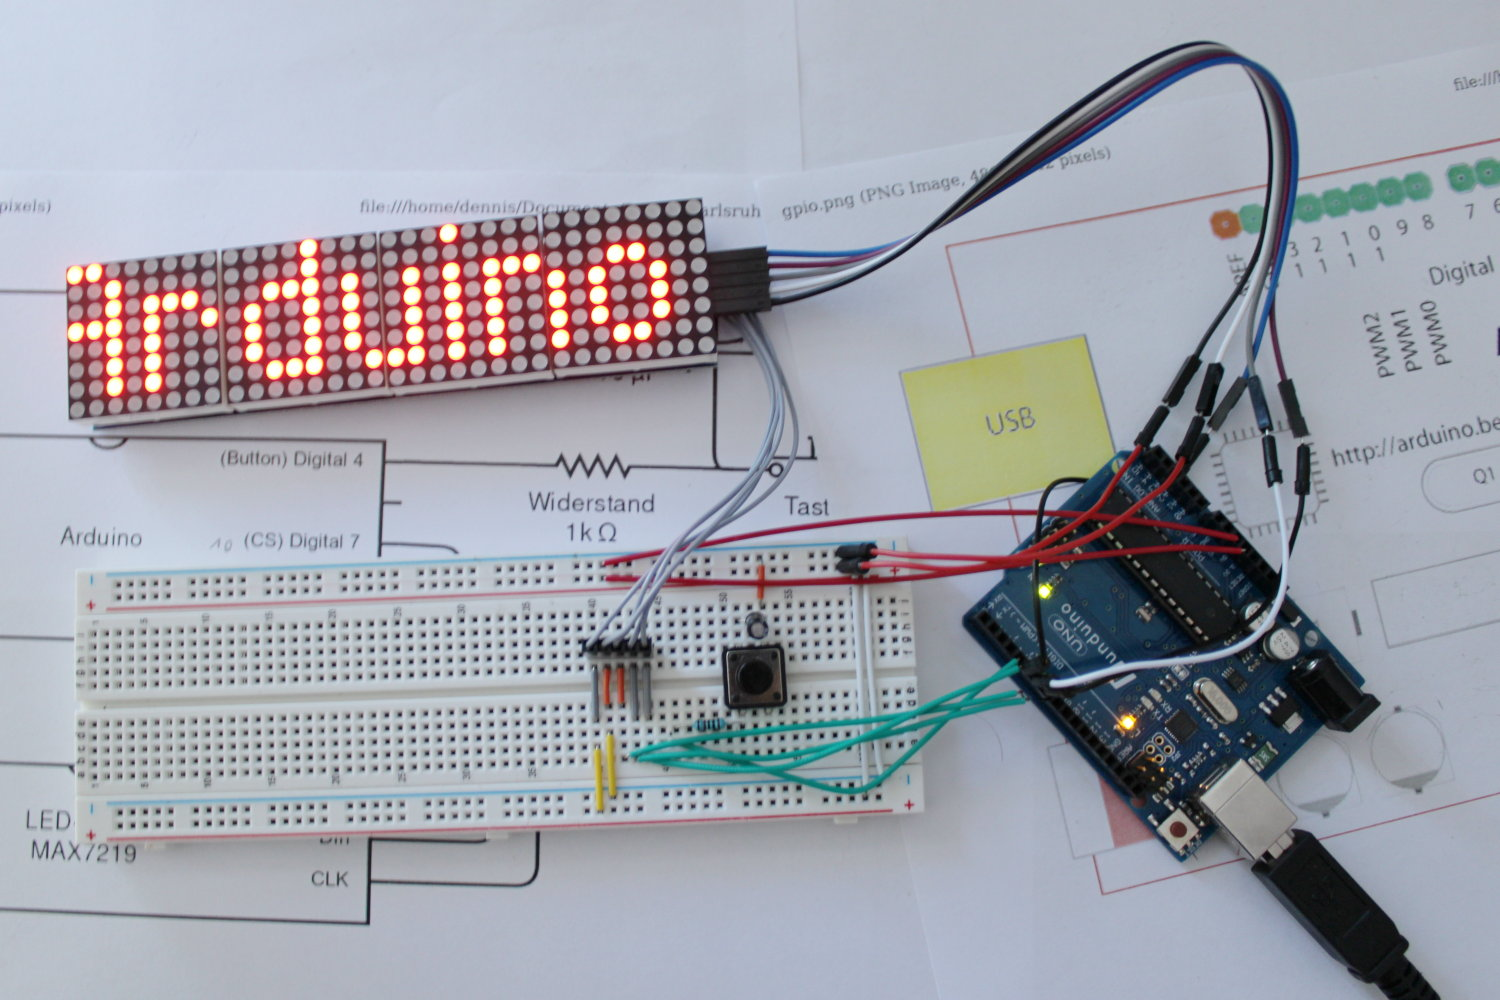
\includegraphics[width=.9\textwidth]{img/laufschrift_arduino1}

        \column{.5\textwidth}
        \textbf{Atmega Microcontroller}
        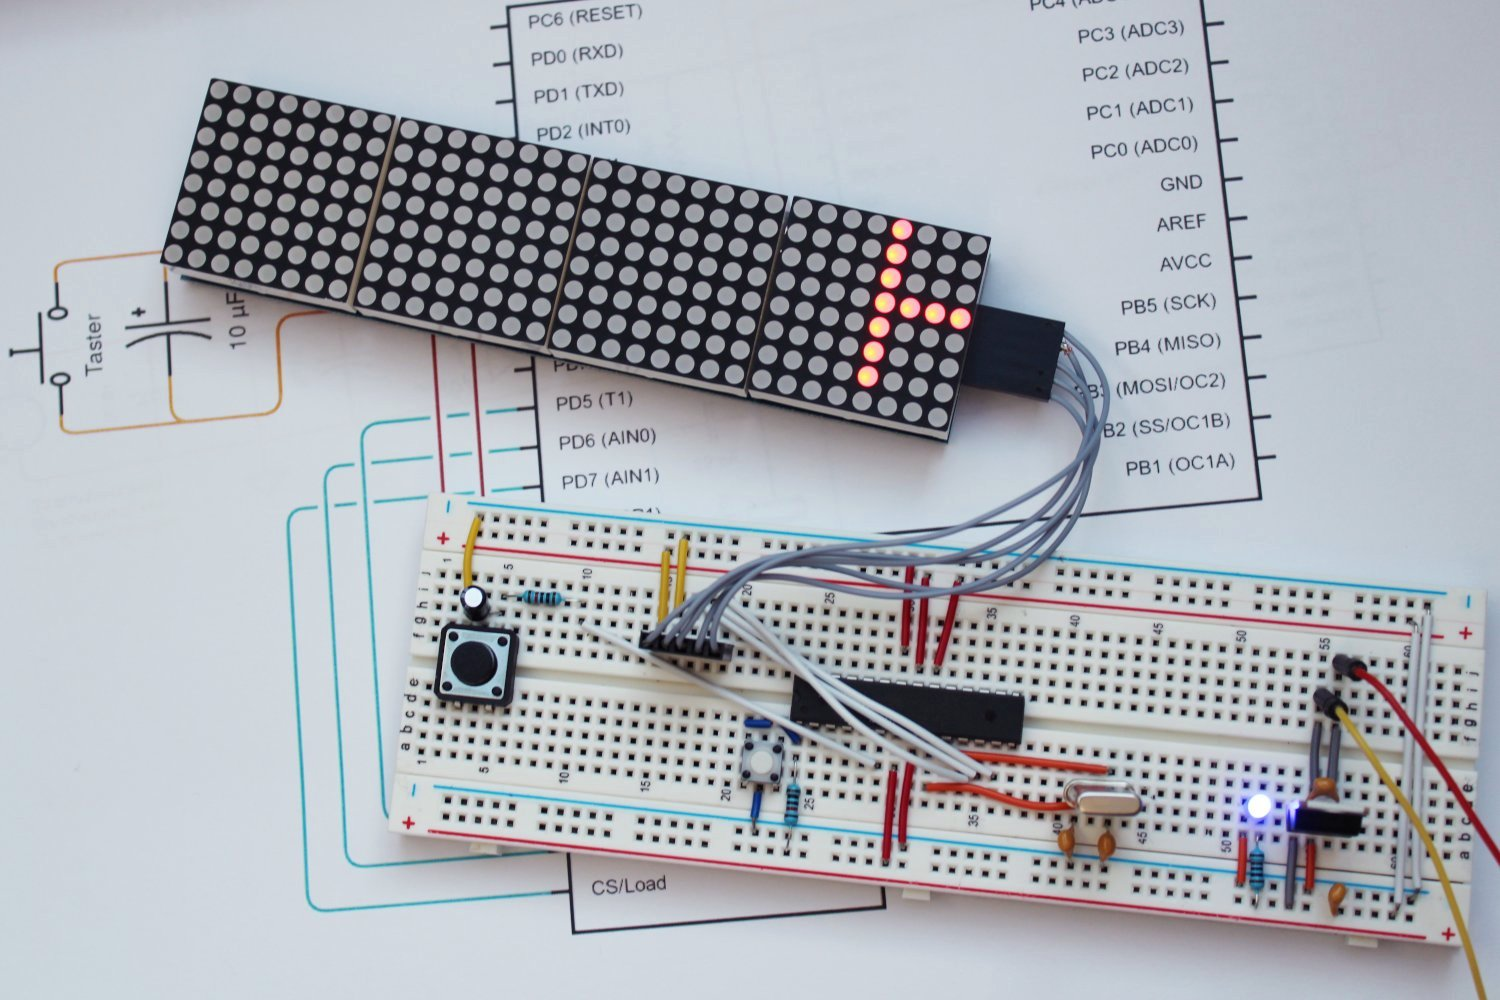
\includegraphics[width=.9\textwidth]{img/laufschrift_arduino2}
    \end{columns}

    \bigskip

    \begin{columns}
        \column{.5\textwidth}
        \textbf{Raspberry Pi auf Breadboard}
        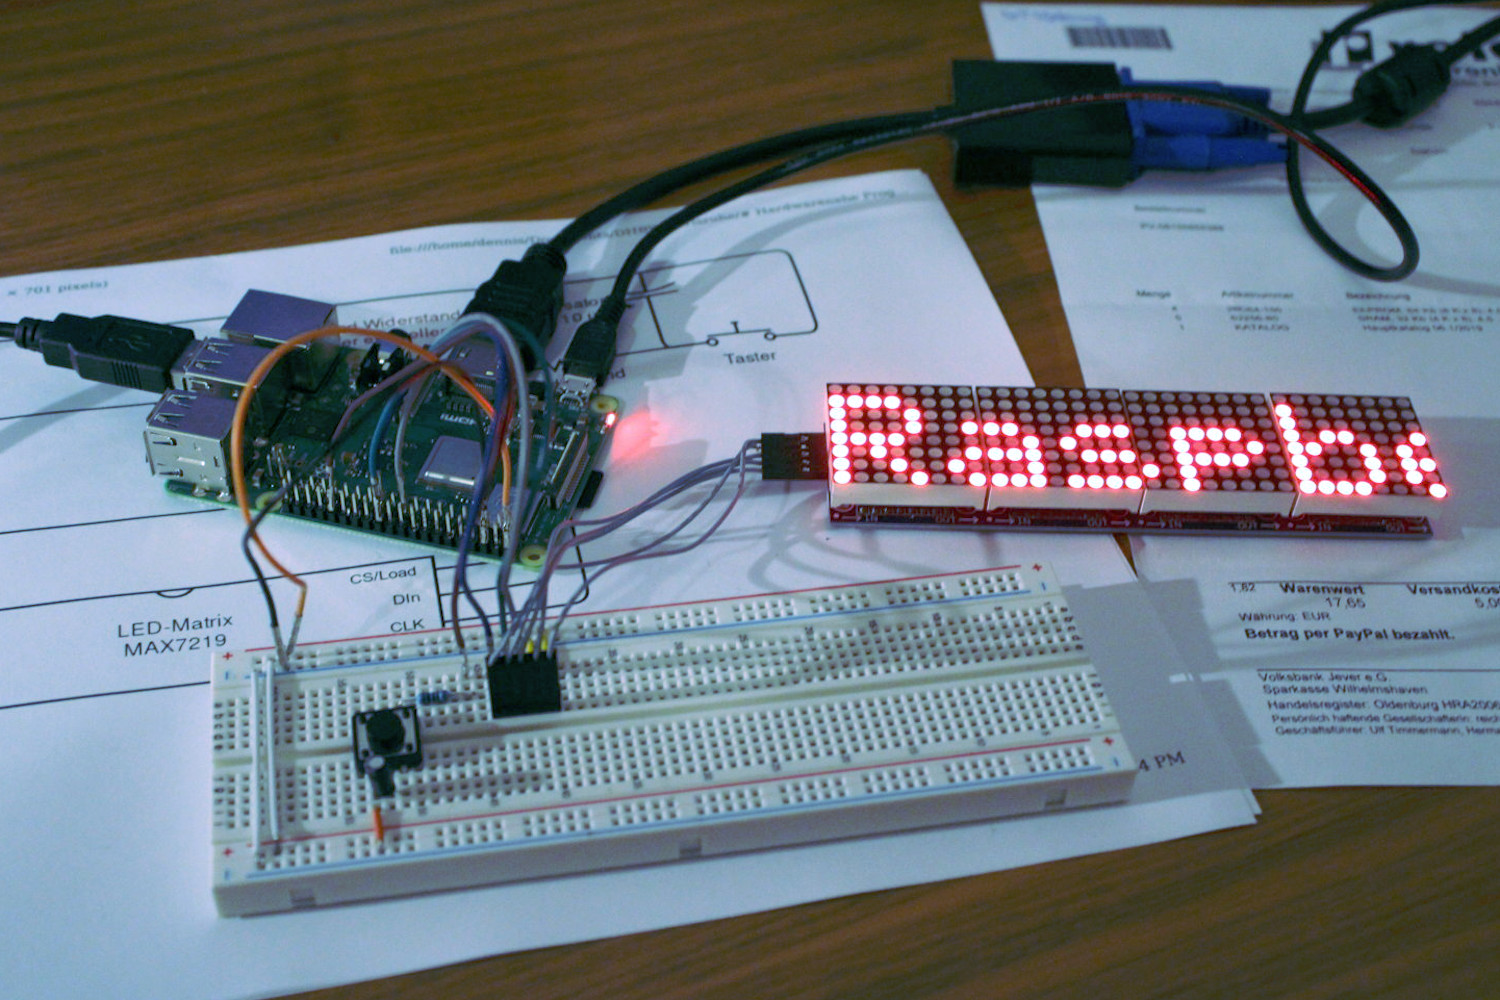
\includegraphics[width=.9\textwidth]{img/laufschrift_pi1}

        \column{.5\textwidth}
        \textbf{Raspberry Pi auf Lochrasterplatine}
        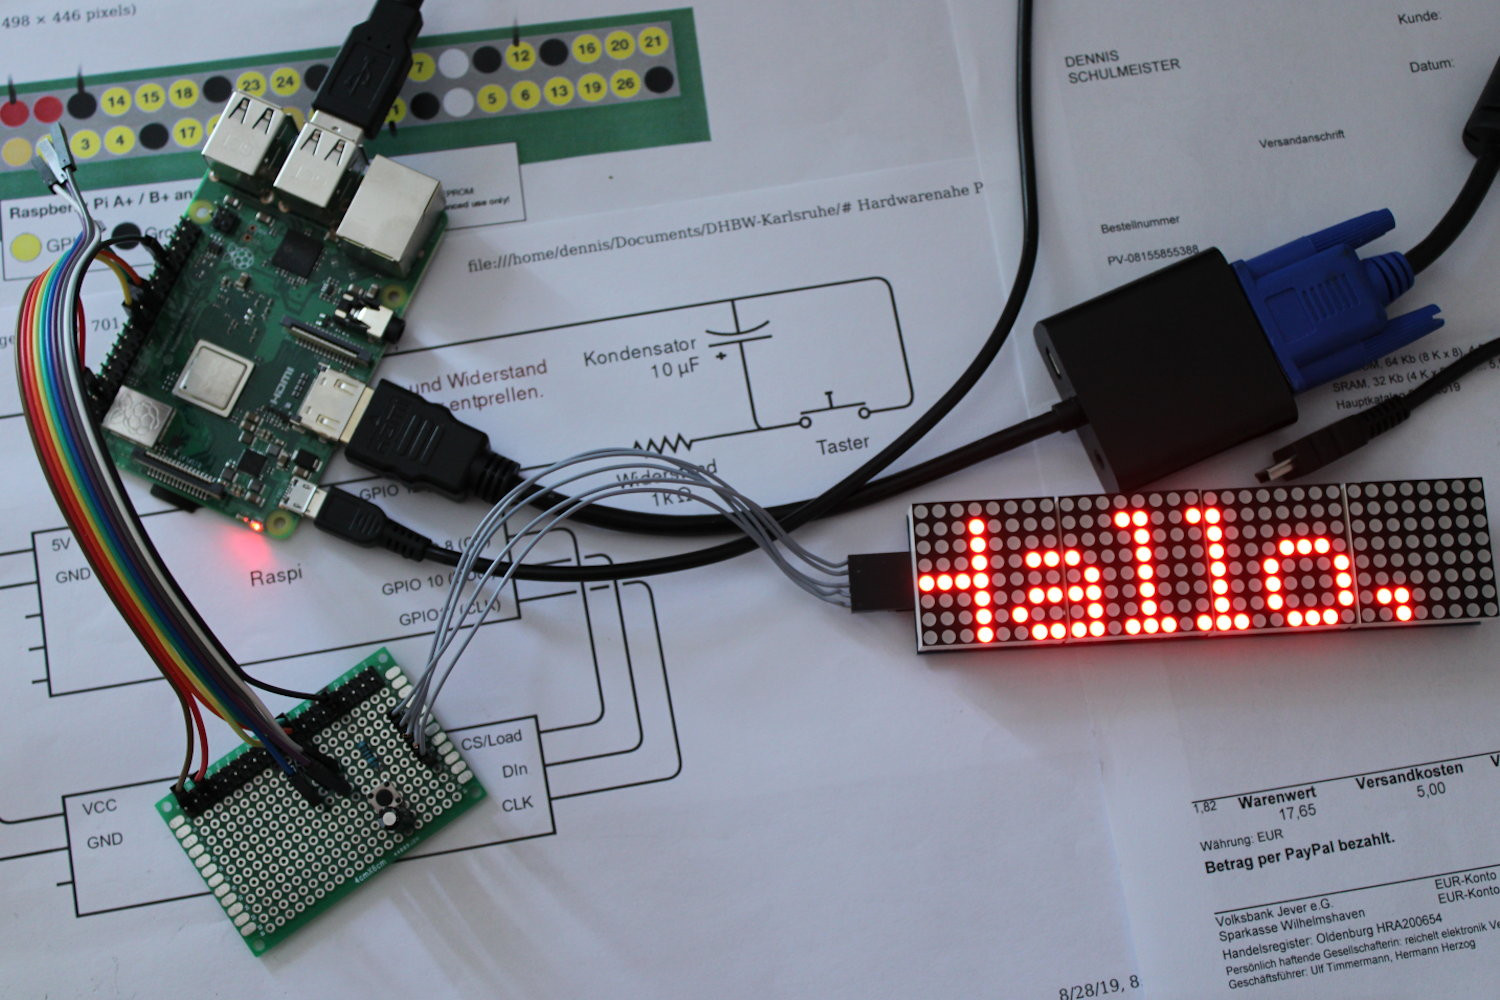
\includegraphics[width=.9\textwidth]{img/laufschrift_pi2}
    \end{columns}
\end{frame}
}

%%% Folie
\begin{frame}[fragile]{Programmierung: Low Level}
    \Justified{
        \footnotesize
        Dass die Architektur \textbf{diskret aufgebauter, eingebetteter Systeme}
        im Grunde genommen die gleiche wie bei \textbf{Microcontroller/SoC-basierten}
        Systemen ist, zeigt sich auch an den Gemeinsamkeiten der hardwarenahen
        Low-Level-Programmierung (hier am Beispiel für AVR).
    }

    \bigskip

    \begin{lstlisting}[language=C, gobble=8]
        #include <avr/io.h>

        int main(void) {
            PORTD |= (1 << PD2);                    // Pull-Up-Widerstand aktivieren
            DDRB = 0xff;                            // Alle Ausgänge an Port B ausschalten

            while (1) {
                if (bit_is_clear(PIND, PD2)) {      // Pin 2 von Port D auf Ground gezogen?
                    PORTB |= 0b10000000;            // Pin 1 von Port B einschalten
                } else {
                    PORTB &= 0b01111111;            // Pin 1 von Port B ausschalten
                }
            }

            return 0;
        }
    \end{lstlisting}

    \bigskip

    \Justified{
        \footnotesize
        Für ARM System-on-a-Chip, wie sie im Rasbperry Pi und vielen anderen Geräten
        genutzt werden, sieht der Code ähnlich aus. Das Geheimnis ist, den richtigen
        Wert an die richtige Speicherstelle zu schreiben, um die Hardware zu steuern.
    }
\end{frame}

%%% Folie
\begin{frame}[fragile]{Programmierung: High Level}
    \Justified{
        \footnotesize
        Aus Gründen der schnelleren und einfacheren Entwicklung sowie der besseren
        Portabilität empfiehlt es sich, zumindest ein einfaches Betriebssystem zu
        nutzen und auf einem höheren Abstraktionsniveu zu programmieren, wenn die
        Systemleistung es zulässt (hier am Beispiel von Python für den Raspberry Pi).
    }

    \smallskip

    \begin{lstlisting}[language=Python, gobble=8, basicstyle=\tiny\ttfamily]
        import os, time
        import RPi.GPIO as GPIO

        GPIO_BUTTON, GPIO_LED = 22, 21

        def on_button_event(button):
            if GPIO.input(button) == GPIO.HIGH:
                GPIO.output(GPIO_LED, True)
            else:
                GPIO.output(GPIO_LED, False)

        if __name__ == "__main__":
            try:
                GPIO.setmode(GPIO.BCM)
                GPIO.setup(GPIO_BUTTON, GPIO.IN, pull_up_down=GPIO.PUD_UP)
                GPIO.setup(GPIO_LED, GPIO.OUT)

                GPIO.add_event_detect(GPIO_BUTTON, GPIO.BOTH)
                GPIO.add_event_callback(GPIO_BUTTON, on_button_event)

                while True:
                    time.sleep(10)
            except KeyboardInterrupt:
                pass

            GPIO.cleanup()
    \end{lstlisting}
\end{frame}

%%% Folie
\begin{frame}{Was nutzen wir in der Vorlesung?}
    \begin{center}
        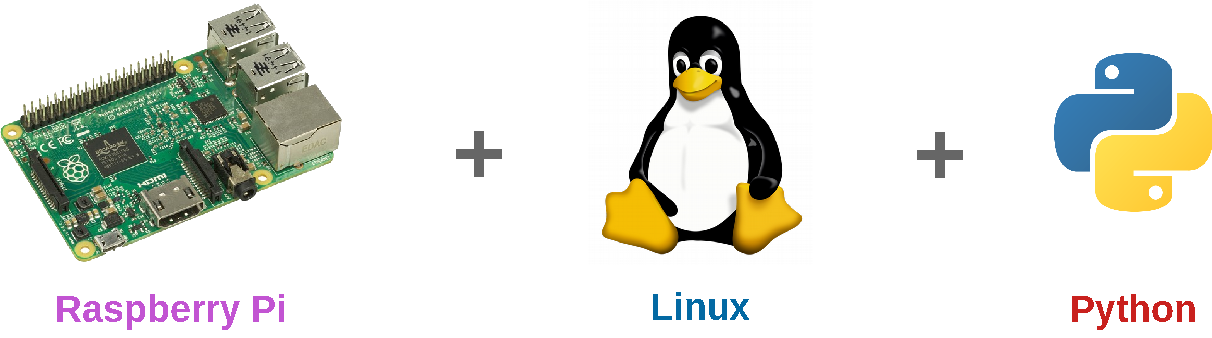
\includegraphics[width=\textwidth]{img/raspi-linux-python}
    \end{center}

    \bigskip

    \Justified{
        \footnotesize
        Wir nutzen eine Kombination aus \textbf{Raspberry Pi}, \textbf{Linux} und
        \textbf{Python}. Sie ist leistungsstark, leicht zu lernen und in der
        IoT-Entwicklung weit verbreitet.

        \medskip

        \begin{itemize}
            \justifying

            \item \textbf{Rasbperry Pi:} Bietet eine vergleichbare Performance wie ein
            älterer Desktopcomputer.

            \item \textbf{Linux:} Beim mitgelieferten Raspberry Pi OS handelt es sich
            um ein angepasstes Debian-Linux. Die meisten Besonderheiten eingebetteter
            Systeme bleiben verborgen, so dass es fast wie ein Desktopsystem nutzbar ist.

            \item \textbf{Python:} Ist eine einsteigerfreundliche Programmiersprache mit
            verschiedenen Anwendungsgebieten. Das Pi in Raspberry Pi stand deshalb ursprünglich
            für ,,Python Interpreter''.
        \end{itemize}
    }
\end{frame}
